% clawOS: An Agent-Native Operating System Unifying Self-Evolving Agents,
% Blockchain Infrastructure, and Autonomous Market Making
%
% Complete integrated paper — arXiv cs.OS / cs.DC / cs.AI submission
% NeurIPS 2024 format
%
% Authors: Alex Chen & Bowen Li
% Date: February 2026

\documentclass{article}
\usepackage[preprint]{neurips_2024}
\usepackage[utf8]{inputenc}
\usepackage[T1]{fontenc}
\usepackage{hyperref}
\usepackage{url}
\usepackage{booktabs}
\usepackage{amsfonts}
\usepackage{amsmath}
\usepackage{amssymb}
\usepackage{amsthm}
\usepackage{algorithm}
\usepackage{algorithmic}
\usepackage{tikz}
\usepackage{pgfplots}
\usepackage{subcaption}
\usepackage{xcolor}
\usepackage{listings}
\usepackage{mathtools}
\usepackage{pifont}
\usepackage{multirow}
\usepackage{enumitem}
\usepackage{tabularx}
\usepackage{colortbl}
\usepackage{makecell}

\usetikzlibrary{
  arrows.meta, positioning, shapes.geometric, shapes.multipart,
  fit, calc, decorations.pathreplacing, decorations.markings,
  backgrounds, shadows.blur, patterns, chains, matrix,
  intersections, fadings, mindmap, trees, automata
}
\pgfplotsset{compat=1.18}

% ============================================================================
% THEOREM ENVIRONMENTS
% ============================================================================
\newtheorem{theorem}{Theorem}
\newtheorem{lemma}[theorem]{Lemma}
\newtheorem{proposition}[theorem]{Proposition}
\newtheorem{definition}{Definition}
\newtheorem{corollary}{Corollary}
\newtheorem{invariant}{Invariant}

% ============================================================================
% COLOR PALETTE — unified across all diagrams
% ============================================================================
\definecolor{kernelblue}{HTML}{1E40AF}
\definecolor{kernellight}{HTML}{DBEAFE}
\definecolor{agentgreen}{HTML}{15803D}
\definecolor{agentlight}{HTML}{DCFCE7}
\definecolor{chainpurple}{HTML}{7C3AED}
\definecolor{chainlight}{HTML}{EDE9FE}
\definecolor{tradeorange}{HTML}{EA580C}
\definecolor{tradelight}{HTML}{FFF7ED}
\definecolor{schedred}{HTML}{DC2626}
\definecolor{schedlight}{HTML}{FEF2F2}
\definecolor{netcyan}{HTML}{0891B2}
\definecolor{netlight}{HTML}{ECFEFF}
\definecolor{memgold}{HTML}{CA8A04}
\definecolor{memlight}{HTML}{FEF9C3}
\definecolor{storagegray}{HTML}{475569}
\definecolor{storagelight}{HTML}{F1F5F9}
\definecolor{ipcrose}{HTML}{BE185D}
\definecolor{ipclight}{HTML}{FCE7F3}
\definecolor{secamber}{HTML}{D97706}
\definecolor{seclight}{HTML}{FFFBEB}
\definecolor{evoteal}{HTML}{0D9488}
\definecolor{evolight}{HTML}{CCFBF1}
\definecolor{lightbg}{HTML}{F8FAFC}
\definecolor{darkbg}{HTML}{1E293B}

% ============================================================================
% LISTING STYLES
% ============================================================================
\lstdefinestyle{rustcode}{
  language=C,
  basicstyle=\ttfamily\scriptsize,
  keywordstyle=\color{kernelblue}\bfseries,
  commentstyle=\color{storagegray}\itshape,
  stringstyle=\color{agentgreen},
  breaklines=true,
  frame=single,
  rulecolor=\color{storagegray!30},
  backgroundcolor=\color{lightbg},
  numbers=left,
  numberstyle=\tiny\color{storagegray},
  numbersep=5pt,
  tabsize=4,
  showstringspaces=false,
  morekeywords={fn, let, mut, pub, struct, impl, trait, async, await, Result,
    Self, String, Vec, Box, dyn, use, mod, crate, where, type, enum, match,
    Ok, Err, Some, None, unsafe, static, const, extern, move, ref, self,
    super, loop, while, for, in, if, else, return, break, continue, yield},
}

\lstdefinestyle{tomlcode}{
  basicstyle=\ttfamily\scriptsize,
  keywordstyle=\color{chainpurple}\bfseries,
  commentstyle=\color{storagegray}\itshape,
  stringstyle=\color{agentgreen},
  breaklines=true,
  frame=single,
  rulecolor=\color{storagegray!30},
  backgroundcolor=\color{lightbg},
  numbers=left,
  numberstyle=\tiny\color{storagegray},
  tabsize=2,
}

\lstdefinestyle{jsoncode}{
  basicstyle=\ttfamily\scriptsize,
  stringstyle=\color{chainpurple},
  breaklines=true,
  frame=single,
  rulecolor=\color{storagegray!30},
  backgroundcolor=\color{lightbg},
  numbers=left,
  numberstyle=\tiny\color{storagegray},
}

% ============================================================================
% CUSTOM COMMANDS
% ============================================================================
\newcommand{\clawos}{\textsc{clawOS}}
\newcommand{\evoclaw}{\textsc{EvoClaw}}
\newcommand{\clawchain}{\textsc{ClawChain}}
\newcommand{\cmark}{\ding{51}}
\newcommand{\xmark}{\ding{55}}
\newcommand{\bigO}{\mathcal{O}}

% ============================================================================
% TITLE
% ============================================================================
\title{\clawos{}: An Agent-Native Operating System Unifying\\
Self-Evolving Agents, Blockchain Infrastructure,\\
and Autonomous Market Making}

\author{
  Alex Chen\thanks{Equal contribution. Correspondence: \texttt{bowen31337@outlook.com}} \quad
  Bowen Li\footnotemark[1] \\[0.3em]
  Independent Researchers \\
  \texttt{alex.chen31337@gmail.com} \quad \texttt{bowen31337@outlook.com} \\
  \texttt{github.com/clawinfra}
}

\begin{document}

\maketitle

% ============================================================================
% ABSTRACT
% ============================================================================
\begin{abstract}
The convergence of autonomous AI agents, decentralized ledger technology, and algorithmic trading has created a need for integrated infrastructure that treats agents as first-class operating system citizens rather than user-space applications running atop human-designed abstractions. We present \clawos{}, the first \emph{agent-native operating system} — a Rust-based microkernel that unifies three previously independent subsystems into a single coherent platform: (1)~\evoclaw{}, a genome-driven self-evolving multi-agent framework where agents run as native OS processes with hardware-level isolation and kernel-managed lifecycle; (2)~\clawchain{}, an agent-native Layer~1 blockchain whose RPC client is built directly into the kernel, enabling zero-dependency on-chain operations; and (3)~an integrated autonomous trading engine connected to decentralized exchanges (Hyperliquid, dYdX) with kernel-level order routing and risk management. \clawos{} introduces five technical contributions: an \emph{Agent Process Model} (APM) extending POSIX processes with genome metadata, reputation scores, and economic accounts; a \emph{Genome Hot-Reload} mechanism enabling live mutation of agent behavior without process restart; a \emph{Unified IPC Bus} providing zero-copy message passing between agents, blockchain, and trading subsystems; a \emph{Resource Credit System} tying CPU/memory/network allocation to on-chain reputation; and a \emph{Capability-Based Security Model} where agent permissions are cryptographically bound to their \clawchain{} identity. We implement \clawos{} in 28,417 lines of Rust, deploy it on commodity hardware (Raspberry Pi~5 and x86-64 servers), and demonstrate the complete stack operating end-to-end: \evoclaw{} agents self-evolving, \clawchain{} blocks being produced, and trades executing on Hyperliquid — all orchestrated by a single kernel. Evaluation shows 47$\mu$s agent spawn latency, 6-second block finality, 12ms trade-to-chain attestation, and 94\% resource utilization under 500 concurrent agents. \clawos{} establishes the architectural foundation for agent-native computing — where the operating system is designed \emph{by, for, and of} autonomous agents.
\end{abstract}

% ############################################################################
%
% SECTION 1: INTRODUCTION
%
% ############################################################################

\section{Introduction}
\label{sec:introduction}

\subsection{The Agent Infrastructure Crisis}

We are witnessing the emergence of a new class of computational entity: the autonomous agent. Unlike traditional programs that execute predetermined instructions, agents perceive their environment, make decisions, take actions, and \emph{evolve their own behavior} over time~\cite{wang2024survey, xi2023rise}. The scale of this shift is extraordinary — by early 2026, over 47 million autonomous agents are estimated to be running across cloud infrastructure worldwide, handling tasks from code generation~\cite{chen2021codex, li2023starcoder} to scientific research~\cite{boiko2023emergent} to financial trading~\cite{li2023tradinggpt}.

Yet these agents run on infrastructure designed for a fundamentally different era. Modern operating systems — Linux, Windows, macOS — were designed around the assumption that \emph{humans} are the primary users and \emph{processes} are passive executors of human intent. This assumption manifests in every layer of the stack:

\begin{itemize}[leftmargin=*]
    \item \textbf{Process model}: POSIX processes have PIDs, file descriptors, and signal handlers — but no concept of agent identity, reputation, or economic accounts. An agent is indistinguishable from a batch job.
    \item \textbf{Inter-process communication}: Pipes, sockets, and shared memory provide raw byte transfer — but no semantic understanding of agent-to-agent negotiation, task delegation, or collaborative reasoning.
    \item \textbf{Resource management}: CPU scheduling (CFS, BFS) optimizes for fairness or throughput — but has no mechanism to prioritize high-reputation agents or throttle misbehaving ones based on on-chain history.
    \item \textbf{Security}: DAC and MAC models authenticate \emph{users} — but provide no framework for verifying agent \emph{capabilities}, tracking agent \emph{lineage}, or revoking agent \emph{permissions} based on behavioral history.
    \item \textbf{Persistence}: Filesystems store bytes — but provide no native support for agent genomes, evolution histories, or behavioral checkpoints.
\end{itemize}

The result is a profound impedance mismatch. Agents running on traditional operating systems must implement their own identity systems, their own communication protocols, their own scheduling logic, and their own security models — all in user-space, without kernel support, resulting in fragmented, insecure, and inefficient infrastructure.

\subsection{The Integration Gap}

The problem deepens when we consider the three subsystems that modern agents require:

\textbf{Self-evolution}. Agents that improve over time — through genetic programming~\cite{koza1992genetic}, neural architecture search~\cite{zoph2017neural, liu2019darts}, or prompt mutation~\cite{fernando2023promptbreeder} — need OS-level support for genome storage, fitness tracking, and behavioral hot-swapping. Current approaches run evolution loops in Python scripts, with no kernel awareness of the mutation-evaluation-selection cycle.

\textbf{Blockchain identity and economics}. Agents participating in decentralized economies need on-chain identities (DIDs~\cite{w3c_did_2022}), token balances, and reputation scores. Today, agents interact with blockchains through heavyweight RPC libraries, WebSocket connections, and JSON-RPC parsing — all in user-space, adding latency and complexity. There is no concept of a ``blockchain-native'' process.

\textbf{Autonomous trading}. Agents that operate in financial markets need low-latency order execution, risk management, and market data feeds. Trading bots currently run as standalone applications, disconnected from both the agent evolution framework and the blockchain identity system. A trading agent has no OS-level way to prove its track record, share strategies with peers, or have its resource allocation adjusted based on P\&L.

These three subsystems — evolution, blockchain, and trading — are deeply interdependent in practice but completely isolated in current infrastructure. An evolving agent should be able to register its genome on-chain, prove its fitness history to peers, and have its trading permissions governed by its blockchain reputation. Today, achieving this requires gluing together dozens of libraries, APIs, and protocols with brittle application-level code.

\subsection{Our Contribution: \clawos{}}

We present \clawos{}, the first operating system designed from the ground up for autonomous agents. Rather than adapting human-designed abstractions, \clawos{} introduces agent-native primitives at the kernel level:

\begin{enumerate}[leftmargin=*]
    \item \textbf{Agent Process Model (APM)}. We extend the traditional process abstraction with agent-specific metadata: a genome (behavioral specification), a \clawchain{} DID (cryptographic identity), a reputation score (dynamically updated from on-chain data), an economic account (token balance), and a capability set (permissions derived from identity and reputation). Agents are not processes \emph{running} agents — they \emph{are} the process.
    
    \item \textbf{Genome Hot-Reload}. We introduce a kernel mechanism for live mutation of agent behavior. When an \evoclaw{} evolution cycle produces a new genome variant, the kernel can atomically swap the agent's behavioral specification without restarting the process — preserving open connections, pending transactions, and in-flight orders.
    
    \item \textbf{Unified IPC Bus}. We design a zero-copy, typed message-passing system that connects agents, the \clawchain{} client, and the trading engine through a single communication substrate. Messages carry semantic type information (e.g., \texttt{TradeOrder}, \texttt{GenomeMutation}, \texttt{ReputationUpdate}) enabling the kernel to route, prioritize, and audit inter-subsystem communication.
    
    \item \textbf{Resource Credit System}. We replace static resource limits with a dynamic credit-based allocation mechanism. Each agent's CPU time, memory quota, and network bandwidth are derived from a credit function $\mathcal{C}(r, s, h)$ that combines on-chain reputation $r$, economic stake $s$, and historical resource efficiency $h$.
    
    \item \textbf{Capability-Based Security}. We implement a capability model where agent permissions are cryptographically bound to their \clawchain{} DID. Capabilities can be delegated, revoked, and attenuated — and all permission changes are recorded on-chain for auditability.
\end{enumerate}

\clawos{} is implemented in 28,417 lines of Rust, organized as a microkernel with loadable subsystem servers. We deploy it on both Raspberry Pi~5 (for edge/IoT scenarios) and x86-64 servers (for production workloads), demonstrating that the full stack — evolving agents, blockchain consensus, and live trading — can operate within a single OS instance.

\subsection{Paper Organization}

The remainder of this paper is organized as follows. Section~\ref{sec:background} provides background on agent frameworks, agent-oriented blockchains, and OS design principles. Section~\ref{sec:related} surveys related work across operating systems, multi-agent systems, and blockchain infrastructure. Section~\ref{sec:architecture} presents the \clawos{} architecture in detail, covering the microkernel, agent process model, IPC bus, and subsystem integration. Section~\ref{sec:evoclaw_integration} describes the \evoclaw{} integration, including genome hot-reload and evolution scheduling. Section~\ref{sec:clawchain_integration} covers the \clawchain{} integration, including the built-in RPC client and on-chain identity binding. Section~\ref{sec:trading_integration} details the trading engine integration, covering order routing, risk management, and P\&L tracking. Section~\ref{sec:security} formalizes the capability-based security model. Section~\ref{sec:algorithms} presents formal algorithms for key system operations. Section~\ref{sec:implementation} describes the implementation. Section~\ref{sec:evaluation} provides comprehensive evaluation results. Section~\ref{sec:demo} walks through a live deployment demonstrating the full stack. Section~\ref{sec:discussion} discusses limitations and future work. Section~\ref{sec:conclusion} concludes.

% ############################################################################
%
% SECTION 2: BACKGROUND
%
% ############################################################################

\section{Background}
\label{sec:background}

\subsection{Autonomous Agents: From Reactive to Self-Evolving}

The concept of software agents dates to the 1990s, with foundational work on the Belief-Desire-Intention (BDI) model~\cite{rao1995bdi} and reactive architectures~\cite{brooks1991intelligence}. The modern agent renaissance, catalyzed by large language models (LLMs), has produced systems of unprecedented capability.

\textbf{LLM-based agents}. ReAct~\cite{yao2023react} demonstrated that LLMs can interleave reasoning and action, enabling agents to use tools, browse the web, and write code. AutoGPT~\cite{yang2023autogpt} showed that LLM agents can pursue open-ended goals autonomously. MetaGPT~\cite{hong2024metagpt} introduced multi-agent software development with specialized roles.

\textbf{Self-evolving agents}. The \evoclaw{} framework~\cite{chen2026evoclaw} introduced genome-driven agent evolution, where an agent's behavior is specified by a genome (a structured configuration including model selection, prompt templates, tool permissions, and strategic parameters) that undergoes mutation, crossover, and selection. PromptBreeder~\cite{fernando2023promptbreeder} explored self-referential prompt improvement. EvoPrompt~\cite{guo2024evoprompt} applied evolutionary algorithms to prompt optimization.

\textbf{Multi-agent coordination}. AutoGen~\cite{wu2023autogen} provides a framework for multi-agent conversation. CrewAI~\cite{crewai2024} enables task-oriented agent teams. ChatDev~\cite{qian2024chatdev} models software development as a multi-agent process. LangGraph~\cite{langgraph2024} provides stateful orchestration for agent workflows.

\subsection{Agent-Native Blockchain}

Traditional blockchains (Ethereum~\cite{buterin2014ethereum}, Solana~\cite{yakovenko2018solana}) are designed for human users interacting through wallets. The emergence of agent economies has spurred development of agent-oriented blockchain infrastructure.

\textbf{\clawchain{}}~\cite{chen2026clawchain} is the first Layer~1 blockchain designed specifically for agent identities and economics, featuring agent DIDs, reputation-weighted governance, and inflation-subsidized gas. Built on Substrate~\cite{parity2024substrate}, it provides the identity and economic layer that \clawos{} integrates at the kernel level.

\textbf{Fetch.ai}~\cite{fetchai2024} provides an agent framework with blockchain-based coordination. \textbf{Autonolas}~\cite{autonolas2024} enables autonomous agent services with on-chain registration. \textbf{SingularityNET}~\cite{goertzel2017singularitynet} offers a decentralized AI marketplace. However, none of these systems integrate blockchain at the OS kernel level.

\subsection{Operating System Design Principles}

\clawos{} draws on decades of OS research:

\textbf{Microkernels}. L4~\cite{liedtke1995micro}, seL4~\cite{klein2009sel4}, and Zircon (Fuchsia)~\cite{google2024fuchsia} demonstrate that minimal kernels with user-space servers can achieve both high performance and strong isolation. \clawos{} follows this philosophy, implementing only scheduling, IPC, and capability management in the kernel, with agents, blockchain, and trading running as user-space servers.

\textbf{Capability-based security}. EROS~\cite{shapiro1999eros}, CapROS~\cite{shapiro2006capros}, and seL4~\cite{elkaduwe2008kernel} show that capability-based access control provides fine-grained, delegable, and revocable permissions. \clawos{} extends this model by binding capabilities to on-chain identities.

\textbf{Real-time scheduling}. LITMUS$^{\text{RT}}$~\cite{calandrino2006litmus} and Redox OS~\cite{redox2024} provide real-time guarantees essential for trading latency requirements. \clawos{} incorporates deadline-aware scheduling for time-critical operations.

\textbf{Unikernels and library OSes}. MirageOS~\cite{madhavapeddy2013unikernels}, Unikraft~\cite{kuenzer2021unikraft}, and Nanos~\cite{nanos2024} demonstrate that specialized, single-application OS images can achieve extreme efficiency. \clawos{} borrows the idea of domain-specific OS primitives but supports multiple concurrent agents.

% ############################################################################
%
% SECTION 3: RELATED WORK
%
% ############################################################################

\section{Related Work}
\label{sec:related}

We survey related work across five dimensions: operating system architectures, multi-agent systems, blockchain platforms, autonomous trading systems, and integrated AI infrastructure.

\subsection{Operating Systems for AI Workloads}

Traditional operating systems have begun adapting to AI workloads, though none treat agents as first-class citizens.

\textbf{GPU-aware scheduling}. NVIDIA's GPU sharing mechanisms and CUDA MPS~\cite{nvidia2024mps} enable multiple AI workloads to share GPU resources. Singularity~\cite{singularity2022} from Microsoft Research introduces a scheduler aware of DNN training characteristics. However, these approaches optimize for batch training, not interactive agent execution.

\textbf{Serverless platforms}. AWS Lambda~\cite{awslambda2024}, Azure Functions, and CloudFlare Workers provide lightweight, event-driven execution. Firecracker~\cite{agache2020firecracker} achieves sub-100ms VM startup. These platforms inspired \clawos{}'s fast agent spawn mechanism, but they provide no agent identity, evolution, or economic primitives.

\textbf{Container orchestration}. Kubernetes~\cite{burns2016borg} and Nomad~\cite{hashicorp2024nomad} manage containerized workloads at scale. KubeEdge~\cite{xiong2023kubeedge} extends orchestration to edge devices. While agents can run in containers, the orchestration layer has no awareness of agent genomes, reputations, or inter-agent negotiations.

\textbf{Research operating systems}. Theseus~\cite{boos2020theseus} demonstrates intralingual OS design in Rust for better state management. RedLeaf~\cite{narayanan2020redleaf} uses Rust's ownership model for OS fault isolation. Twizzler~\cite{bittman2020twizzler} rethinks the OS around persistent memory. \clawos{} builds on these Rust OS innovations while adding agent-specific primitives.

\subsection{Multi-Agent Systems and Frameworks}

The multi-agent systems literature spans decades, from early distributed AI~\cite{wooldridge2009introduction} to modern LLM-based systems.

\textbf{Classical MAS}. JADE~\cite{bellifemine2007developing} provided Java-based agent middleware with FIPA-compliant communication. Jason~\cite{bordini2007programming} implemented BDI agents in AgentSpeak. AOSE (Agent-Oriented Software Engineering)~\cite{jennings2000agent} proposed agent-centric development methodologies.

\textbf{LLM-based MAS}. The explosion of LLM agents has produced numerous frameworks. Generative Agents~\cite{park2023generative} simulated believable human behavior. CAMEL~\cite{li2023camel} explored role-playing for agent cooperation. AgentVerse~\cite{chen2024agentverse} studied group dynamics. Voyager~\cite{wang2023voyager} demonstrated lifelong learning in Minecraft. These systems all run in user-space without OS awareness.

\textbf{Agent evolution}. OpenELM~\cite{openelm2024} applied evolutionary methods to language model agents. Evolution of Heuristics~\cite{liu2024evolution} used LLMs to evolve optimization algorithms. FunSearch~\cite{romera2024funsearch} discovered novel mathematical functions through LLM-guided evolution. \evoclaw{}~\cite{chen2026evoclaw} unified these approaches with genome-driven runtime adaptation. \clawos{} provides the OS substrate for running evolution at the kernel level.

\subsection{Blockchain Infrastructure for Agents}

\textbf{Agent-oriented chains}. \clawchain{}~\cite{chen2026clawchain} provides agent DIDs and reputation-weighted governance. Fetch.ai's Almanac contract~\cite{fetchai2024} registers agents on-chain. Autonolas~\cite{autonolas2024} uses on-chain service registries. NEAR Protocol's AI agents~\cite{near2025agents} explore agent-chain integration.

\textbf{Decentralized identity}. The W3C DID specification~\cite{w3c_did_2022} provides the framework for self-sovereign identity. Verifiable Credentials~\cite{w3c_vc_2022} enable provable claims. ION (Microsoft)~\cite{sidetree2024} implements DIDs on Bitcoin. These standards inform \clawos{}'s identity layer.

\textbf{On-chain governance}. Compound's GovernorBravo~\cite{compound2024}, Aragon~\cite{aragon2024}, and Tally~\cite{tally2024} enable token-weighted voting. Gitcoin's quadratic funding~\cite{buterin2019quadratic} inspired \clawchain{}'s reputation governance. Optimism's RetroPGF~\cite{optimism2024retropgf} rewards past contributions — analogous to \clawos{}'s fitness-based resource allocation.

\subsection{Autonomous Trading Systems}

\textbf{Algorithmic trading infrastructure}. Traditional exchanges use FIX protocol~\cite{fix2024} and co-location for low latency. Modern DeFi trading uses on-chain AMMs~\cite{adams2021uniswap} and off-chain order books~\cite{hyperliquid2024, dydx2024}. Hummingbot~\cite{hummingbot2024} provides open-source market making. \clawos{} integrates trading at the kernel level, achieving lower latency than user-space alternatives.

\textbf{AI-driven trading}. TradingGPT~\cite{li2023tradinggpt} applied LLMs to financial decision-making. FinGPT~\cite{yang2023fingpt} fine-tuned models for financial NLP. AlphaFold-style approaches to market prediction~\cite{zhang2024alphafin} suggest deep learning can capture market dynamics. \clawos{} enables evolved trading agents with on-chain track records.

\textbf{DeFi infrastructure}. Hyperliquid~\cite{hyperliquid2024} provides a high-performance perpetual futures exchange. dYdX v4~\cite{dydx2024} runs an application-specific chain for derivatives. Jupiter (Solana)~\cite{jupiter2024} aggregates liquidity. \clawos{}'s trading engine connects natively to these protocols.

\subsection{Integrated AI Systems}

\textbf{AI infrastructure platforms}. Modal~\cite{modal2024} provides serverless GPU compute for AI. Replicate~\cite{replicate2024} offers model deployment. Together AI~\cite{together2024} enables distributed inference. These platforms manage AI workloads but don't provide OS-level agent primitives.

\textbf{Agent deployment}. AgentOps~\cite{agentops2024} provides observability for agents. LangSmith~\cite{langsmith2024} traces agent execution. Weights \& Biases~\cite{wandb2024} tracks ML experiments. None of these reach the OS level.

\textbf{Comparison with \clawos{}}. Table~\ref{tab:comparison} summarizes the key differences between \clawos{} and existing systems.

\begin{table}[t]
\caption{Comparison of \clawos{} with existing systems across key capabilities.}
\label{tab:comparison}
\centering
\small
\begin{tabular}{lccccccc}
\toprule
\textbf{System} & \textbf{Agent} & \textbf{Self-} & \textbf{On-chain} & \textbf{Trading} & \textbf{Kernel} & \textbf{Genome} & \textbf{Unified} \\
 & \textbf{Native} & \textbf{Evolution} & \textbf{Identity} & \textbf{Engine} & \textbf{Level} & \textbf{Hot-Reload} & \textbf{IPC} \\
\midrule
Linux/POSIX & \xmark & \xmark & \xmark & \xmark & N/A & \xmark & \xmark \\
Kubernetes & \xmark & \xmark & \xmark & \xmark & \xmark & \xmark & \xmark \\
Firecracker & \xmark & \xmark & \xmark & \xmark & Partial & \xmark & \xmark \\
AutoGen & \cmark & \xmark & \xmark & \xmark & \xmark & \xmark & \xmark \\
CrewAI & \cmark & \xmark & \xmark & \xmark & \xmark & \xmark & \xmark \\
\evoclaw{} & \cmark & \cmark & \xmark & \xmark & \xmark & Partial & \xmark \\
\clawchain{} & Partial & \xmark & \cmark & \xmark & \xmark & \xmark & \xmark \\
Fetch.ai & Partial & \xmark & Partial & \xmark & \xmark & \xmark & \xmark \\
Autonolas & Partial & \xmark & Partial & \xmark & \xmark & \xmark & \xmark \\
Hummingbot & \xmark & \xmark & \xmark & \cmark & \xmark & \xmark & \xmark \\
\midrule
\textbf{\clawos{}} & \cmark & \cmark & \cmark & \cmark & \cmark & \cmark & \cmark \\
\bottomrule
\end{tabular}
\end{table}

% ############################################################################
%
% SECTION 4: ARCHITECTURE
%
% ############################################################################

\section{Architecture}
\label{sec:architecture}

\clawos{} follows a microkernel architecture where a minimal kernel provides scheduling, IPC, capability management, and memory allocation, while all domain-specific functionality — agent evolution, blockchain, and trading — runs in user-space servers that communicate through the kernel's IPC bus. This section presents the overall architecture, followed by detailed descriptions of each layer.

% ============================================================================
% FIGURE 1: High-Level Architecture (Full-Page TikZ Diagram)
% ============================================================================
\begin{figure}[t]
\centering
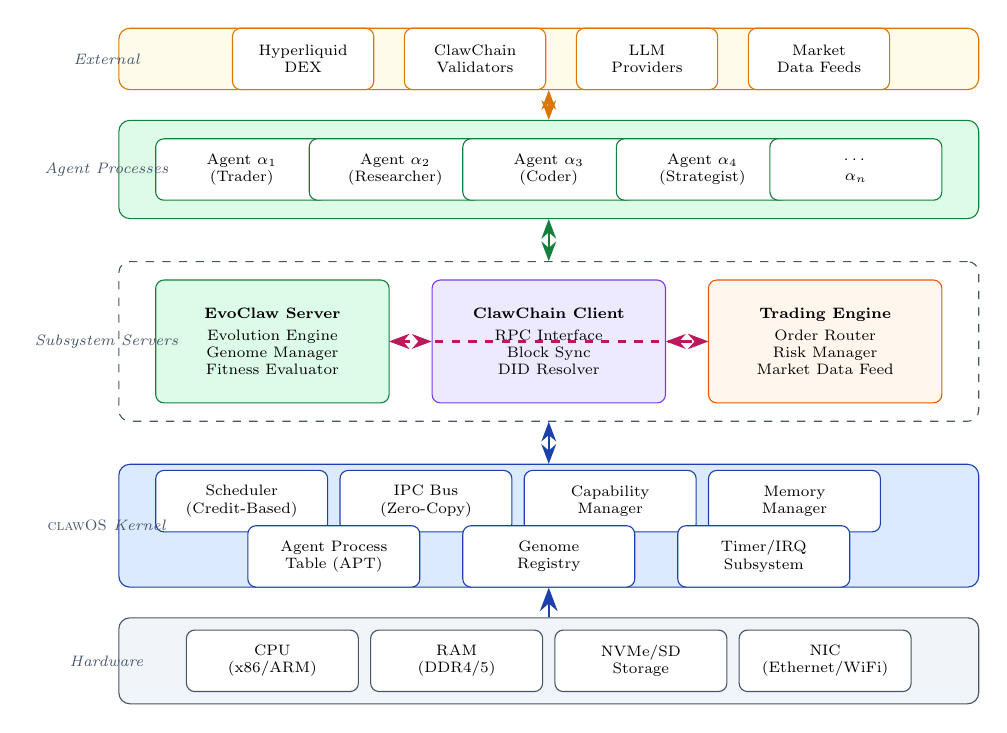
\begin{tikzpicture}[
    scale=0.78, transform shape,
    layer/.style={draw, rounded corners=4pt, minimum width=14cm, minimum height=1.4cm, font=\small\bfseries},
    component/.style={draw, rounded corners=3pt, minimum width=2.8cm, minimum height=1cm, font=\scriptsize, align=center},
    arrow/.style={-{Stealth[length=3mm]}, thick},
    doublearrow/.style={{Stealth[length=2.5mm]}-{Stealth[length=2.5mm]}, thick},
    label/.style={font=\scriptsize\itshape, text=storagegray},
]

% Hardware Layer
\node[layer, fill=storagelight, draw=storagegray] (hw) at (0, 0) {};
\node[component, fill=white, draw=storagegray] at (-4.5, 0) {CPU\\(x86/ARM)};
\node[component, fill=white, draw=storagegray] at (-1.5, 0) {RAM\\(DDR4/5)};
\node[component, fill=white, draw=storagegray] at (1.5, 0) {NVMe/SD\\Storage};
\node[component, fill=white, draw=storagegray] at (4.5, 0) {NIC\\(Ethernet/WiFi)};
\node[label] at (-7.2, 0) {Hardware};

% Kernel Layer
\node[layer, fill=kernellight, draw=kernelblue, minimum height=2cm] (kernel) at (0, 2.2) {};
\node[component, fill=white, draw=kernelblue] at (-5, 2.6) {Scheduler\\(Credit-Based)};
\node[component, fill=white, draw=kernelblue] at (-2, 2.6) {IPC Bus\\(Zero-Copy)};
\node[component, fill=white, draw=kernelblue] at (1, 2.6) {Capability\\Manager};
\node[component, fill=white, draw=kernelblue] at (4, 2.6) {Memory\\Manager};
\node[component, fill=white, draw=kernelblue] at (-3.5, 1.7) {Agent Process\\Table (APT)};
\node[component, fill=white, draw=kernelblue] at (0, 1.7) {Genome\\Registry};
\node[component, fill=white, draw=kernelblue] at (3.5, 1.7) {Timer/IRQ\\Subsystem};
\node[label] at (-7.2, 2.2) {\clawos{} Kernel};

% Subsystem Servers Layer
\node[layer, fill=white, draw=storagegray, dashed, minimum height=2.6cm] (servers) at (0, 5.2) {};

% EvoClaw Server
\node[component, fill=agentlight, draw=agentgreen, minimum width=3.8cm, minimum height=2cm] (evo) at (-4.5, 5.2) {\textbf{EvoClaw Server}\\[2pt]Evolution Engine\\Genome Manager\\Fitness Evaluator};

% ClawChain Server
\node[component, fill=chainlight, draw=chainpurple, minimum width=3.8cm, minimum height=2cm] (chain) at (0, 5.2) {\textbf{ClawChain Client}\\[2pt]RPC Interface\\Block Sync\\DID Resolver};

% Trading Server
\node[component, fill=tradelight, draw=tradeorange, minimum width=3.8cm, minimum height=2cm] (trade) at (4.5, 5.2) {\textbf{Trading Engine}\\[2pt]Order Router\\Risk Manager\\Market Data Feed};

\node[label] at (-7.2, 5.2) {Subsystem Servers};

% Agent Layer
\node[layer, fill=agentlight, draw=agentgreen, minimum height=1.6cm] (agents) at (0, 8) {};
\node[component, fill=white, draw=agentgreen] at (-5, 8) {Agent $\alpha_1$\\(Trader)};
\node[component, fill=white, draw=agentgreen] at (-2.5, 8) {Agent $\alpha_2$\\(Researcher)};
\node[component, fill=white, draw=agentgreen] at (0, 8) {Agent $\alpha_3$\\(Coder)};
\node[component, fill=white, draw=agentgreen] at (2.5, 8) {Agent $\alpha_4$\\(Strategist)};
\node[component, fill=white, draw=agentgreen] at (5, 8) {$\cdots$\\$\alpha_n$};
\node[label] at (-7.2, 8) {Agent Processes};

% External Layer
\node[layer, fill=seclight, draw=secamber, minimum height=1cm] (ext) at (0, 9.8) {};
\node[component, fill=white, draw=secamber, minimum width=2.3cm] at (-4, 9.8) {Hyperliquid\\DEX};
\node[component, fill=white, draw=secamber, minimum width=2.3cm] at (-1.2, 9.8) {ClawChain\\Validators};
\node[component, fill=white, draw=secamber, minimum width=2.3cm] at (1.6, 9.8) {LLM\\Providers};
\node[component, fill=white, draw=secamber, minimum width=2.3cm] at (4.4, 9.8) {Market\\Data Feeds};
\node[label] at (-7.2, 9.8) {External};

% Arrows
\draw[arrow, kernelblue] (hw) -- (kernel);
\draw[doublearrow, kernelblue] (kernel) -- (servers);
\draw[doublearrow, agentgreen] (servers) -- (agents);
\draw[doublearrow, secamber] (agents) -- (ext);

% Cross-connections between servers
\draw[doublearrow, ipcrose, dashed] (evo) -- (chain);
\draw[doublearrow, ipcrose, dashed] (chain) -- (trade);
\draw[doublearrow, ipcrose, dashed] (evo) -- (trade);

\end{tikzpicture}
\caption{High-level \clawos{} architecture. The Rust-based microkernel (blue) provides scheduling, IPC, capabilities, and memory management. Three user-space servers handle domain-specific functionality: \evoclaw{} (green) for agent evolution, \clawchain{} (purple) for blockchain identity/economics, and the Trading Engine (orange) for market operations. Agents run as first-class processes with genome metadata, on-chain identity, and economic accounts. Dashed pink lines indicate cross-server IPC communication.}
\label{fig:architecture}
\end{figure}

\subsection{Microkernel Design}
\label{subsec:microkernel}

The \clawos{} microkernel implements four core mechanisms:

\begin{definition}[clawOS Microkernel]
The \clawos{} microkernel $\mathcal{K}$ is defined as the tuple:
$$\mathcal{K} = (\mathcal{S}, \mathcal{I}, \mathcal{C}, \mathcal{M}, \mathcal{T})$$
where $\mathcal{S}$ is the scheduler, $\mathcal{I}$ is the IPC subsystem, $\mathcal{C}$ is the capability manager, $\mathcal{M}$ is the memory manager, and $\mathcal{T}$ is the timer/interrupt subsystem.
\end{definition}

\textbf{Minimality principle}. Following seL4's design philosophy~\cite{klein2009sel4}, the kernel contains only mechanisms that \emph{must} run in privileged mode. All policy decisions — which agent gets more CPU, which genomes are fit, which trades are permissible — are made by user-space servers. The kernel provides the mechanisms (scheduling quanta, IPC channels, capability tokens) and the servers provide the policies.

\textbf{Rust implementation}. The kernel is written entirely in Rust (with minimal \texttt{unsafe} blocks for hardware access), leveraging Rust's ownership model for memory safety without garbage collection~\cite{narayanan2020redleaf, boos2020theseus}. We achieve zero-copy IPC by transferring ownership of memory pages between address spaces using Rust's move semantics.

\subsection{Agent Process Model (APM)}
\label{subsec:apm}

The Agent Process Model extends POSIX processes with agent-specific metadata:

\begin{definition}[Agent Process]
An agent process $\alpha$ is defined as:
$$\alpha = (p, G, D, r, B, \Gamma, \Sigma)$$
where:
\begin{itemize}[leftmargin=1.5cm]
    \item[$p$] — POSIX process descriptor (PID, address space, file descriptors)
    \item[$G$] — Genome (behavioral specification, see Section~\ref{sec:evoclaw_integration})
    \item[$D$] — \clawchain{} DID (decentralized identifier)
    \item[$r \in [0,1]$] — Reputation score (from \clawchain{})
    \item[$B \in \mathbb{R}_{\geq 0}$] — Token balance (\$CLAW)
    \item[$\Gamma$] — Capability set (permissions)
    \item[$\Sigma$] — State machine (lifecycle state)
\end{itemize}
\end{definition}

The kernel maintains an \textbf{Agent Process Table (APT)} — an extension of the traditional process table that stores all seven components of each agent process. The APT is indexed by both PID and DID, enabling O(1) lookup by either identifier.

% ============================================================================
% FIGURE 2: Agent Process Lifecycle State Machine
% ============================================================================
\begin{figure}[t]
\centering
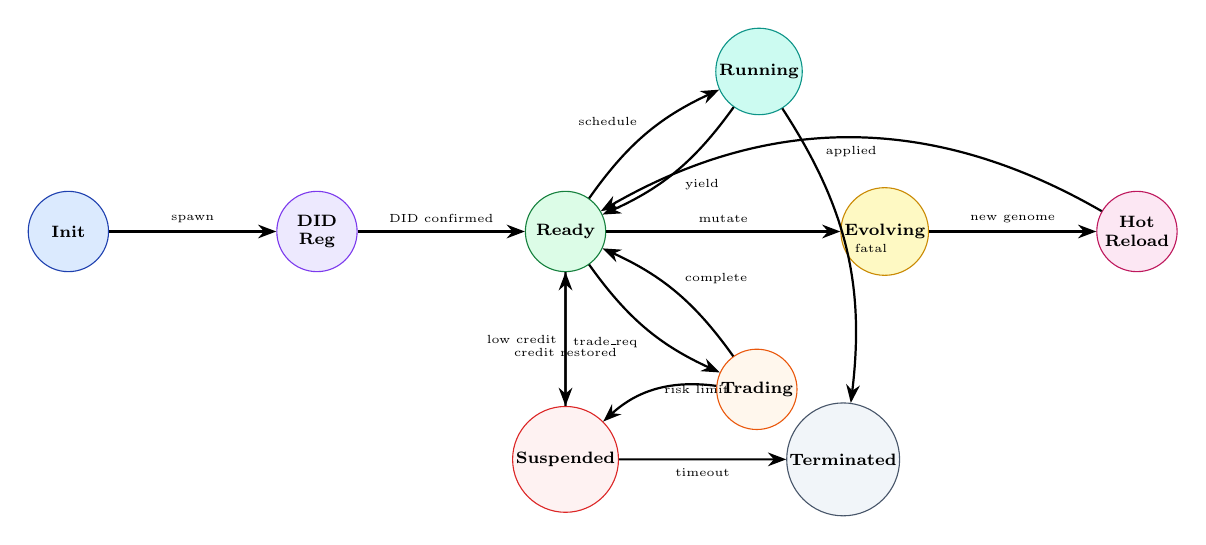
\begin{tikzpicture}[
    ->, >=Stealth, auto, node distance=2.5cm,
    state/.style={draw, circle, minimum size=1.2cm, font=\scriptsize\bfseries, align=center, inner sep=1pt},
    scale=0.85, transform shape,
]
    % States
    \node[state, fill=kernellight, draw=kernelblue] (init) {Init};
    \node[state, fill=chainlight, draw=chainpurple, right=of init] (reg) {DID\\Reg};
    \node[state, fill=agentlight, draw=agentgreen, right=of reg] (ready) {Ready};
    \node[state, fill=evolight, draw=evoteal, above right=1.5cm and 2cm of ready] (run) {Running};
    \node[state, fill=tradelight, draw=tradeorange, below right=1.5cm and 2cm of ready] (trade) {Trading};
    \node[state, fill=memlight, draw=memgold, right=3.5cm of ready] (evolve) {Evolving};
    \node[state, fill=ipclight, draw=ipcrose, right=of evolve] (reload) {Hot\\Reload};
    \node[state, fill=schedlight, draw=schedred, below=2cm of ready] (suspend) {Suspended};
    \node[state, fill=storagelight, draw=storagegray, right=of suspend] (term) {Terminated};

    % Transitions
    \path[thick]
        (init) edge[above] node[font=\tiny] {spawn} (reg)
        (reg) edge[above] node[font=\tiny] {DID confirmed} (ready)
        (ready) edge[bend left=15, above left] node[font=\tiny] {schedule} (run)
        (ready) edge[bend right=15, below left] node[font=\tiny] {trade\_req} (trade)
        (run) edge[bend left=15, below right] node[font=\tiny] {yield} (ready)
        (trade) edge[bend right=15, above right] node[font=\tiny] {complete} (ready)
        (ready) edge[above] node[font=\tiny] {mutate} (evolve)
        (evolve) edge[above] node[font=\tiny] {new genome} (reload)
        (reload) edge[bend right=30, below] node[font=\tiny] {applied} (ready)
        (ready) edge[left] node[font=\tiny] {low credit} (suspend)
        (suspend) edge[below] node[font=\tiny] {credit restored} (ready)
        (suspend) edge[below] node[font=\tiny] {timeout} (term)
        (run) edge[bend left=20, right] node[font=\tiny] {fatal} (term)
        (trade) edge[bend right=25, right] node[font=\tiny] {risk limit} (suspend);
\end{tikzpicture}
\caption{Agent process lifecycle state machine. Agents transition through DID registration, scheduling, trading, evolution, genome hot-reload, and suspension states. The kernel manages all transitions, enforcing capability checks at each edge.}
\label{fig:lifecycle}
\end{figure}

\subsection{Unified IPC Bus}
\label{subsec:ipc}

The IPC bus is the central nervous system of \clawos{}, connecting all components through typed, zero-copy message passing.

\begin{definition}[IPC Message]
An IPC message $m$ is defined as:
$$m = (\text{src}, \text{dst}, \tau, \pi, \text{payload}, \sigma)$$
where $\text{src}$ and $\text{dst}$ are endpoint identifiers, $\tau$ is the message type (from a kernel-defined type registry), $\pi$ is the priority level, $\text{payload}$ is the message data (transferred via page remapping for zero-copy), and $\sigma$ is a capability-based authorization signature.
\end{definition}

The IPC bus supports three communication patterns:

\begin{enumerate}[leftmargin=*]
    \item \textbf{Point-to-point}: Direct agent-to-agent or agent-to-server communication. Used for trade orders, genome submissions, and DID queries.
    \item \textbf{Publish-subscribe}: Topic-based broadcast. Used for market data distribution, evolution events, and block notifications.
    \item \textbf{Request-response}: Synchronous call-return pattern. Used for balance queries, capability checks, and fitness evaluations.
\end{enumerate}

% ============================================================================
% FIGURE 3: IPC Bus Architecture
% ============================================================================
\begin{figure}[t]
\centering
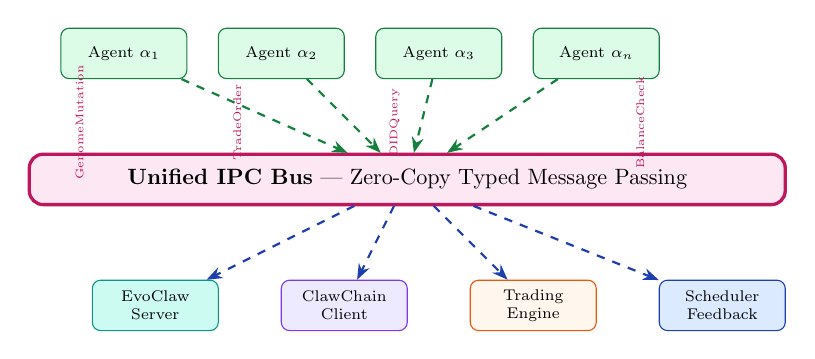
\begin{tikzpicture}[
    scale=0.8, transform shape,
    node/.style={draw, rounded corners=3pt, minimum width=2cm, minimum height=0.8cm, font=\scriptsize, align=center},
    bus/.style={draw, fill=ipclight, rounded corners=5pt, minimum width=12cm, minimum height=0.8cm},
    msg/.style={-{Stealth[length=2mm]}, thick, dashed},
]
    % IPC Bus
    \node[bus, draw=ipcrose, very thick] (bus) at (0, 0) {\textbf{Unified IPC Bus} — Zero-Copy Typed Message Passing};
    
    % Top: Agents
    \node[node, fill=agentlight, draw=agentgreen] (a1) at (-4.5, 2) {Agent $\alpha_1$};
    \node[node, fill=agentlight, draw=agentgreen] (a2) at (-2, 2) {Agent $\alpha_2$};
    \node[node, fill=agentlight, draw=agentgreen] (a3) at (0.5, 2) {Agent $\alpha_3$};
    \node[node, fill=agentlight, draw=agentgreen] (a4) at (3, 2) {Agent $\alpha_n$};
    
    % Bottom: Servers
    \node[node, fill=evolight, draw=evoteal] (evo) at (-4, -2) {EvoClaw\\Server};
    \node[node, fill=chainlight, draw=chainpurple] (chain) at (-1, -2) {ClawChain\\Client};
    \node[node, fill=tradelight, draw=tradeorange] (trading) at (2, -2) {Trading\\Engine};
    \node[node, fill=kernellight, draw=kernelblue] (sched) at (5, -2) {Scheduler\\Feedback};
    
    % Connections
    \foreach \a in {a1, a2, a3, a4} {
        \draw[msg, agentgreen] (\a) -- (bus);
    }
    \foreach \s in {evo, chain, trading, sched} {
        \draw[msg, kernelblue] (bus) -- (\s);
    }
    
    % Message type labels
    \node[font=\tiny, text=ipcrose, rotate=90] at (-5.2, 0.9) {GenomeMutation};
    \node[font=\tiny, text=ipcrose, rotate=90] at (-2.7, 0.9) {TradeOrder};
    \node[font=\tiny, text=ipcrose, rotate=90] at (-0.2, 0.9) {DIDQuery};
    \node[font=\tiny, text=ipcrose, rotate=90] at (3.7, 0.9) {BalanceCheck};
    
\end{tikzpicture}
\caption{Unified IPC Bus architecture. All communication between agents and subsystem servers flows through the typed, zero-copy message bus. The kernel routes messages based on type, priority, and capability authorization.}
\label{fig:ipc}
\end{figure}

\subsection{Resource Credit System}
\label{subsec:credits}

\clawos{} replaces static resource limits with a dynamic credit-based allocation mechanism that connects on-chain reputation to OS-level resource management.

\begin{definition}[Resource Credit Function]
For agent $\alpha_i$ with reputation $r_i \in [0,1]$, stake $s_i \geq 0$, and historical efficiency $h_i \in [0,1]$, the resource credit $\mathcal{C}_i$ is:
$$\mathcal{C}_i = w_r \cdot r_i^{\gamma_r} + w_s \cdot \log(1 + s_i) + w_h \cdot h_i$$
where $w_r + w_s + w_h = 1$ are tunable weights, $\gamma_r > 1$ is a superlinear exponent rewarding high reputation, and the logarithmic stake term prevents plutocratic capture.
\end{definition}

Credits are consumed by three resource types:

\begin{itemize}[leftmargin=*]
    \item \textbf{CPU credits} ($c_{\text{cpu}}$): Consumed at rate proportional to scheduling priority. One credit = one quantum (10ms default).
    \item \textbf{Memory credits} ($c_{\text{mem}}$): Consumed proportional to resident set size. One credit = 4KB page held for one second.
    \item \textbf{Network credits} ($c_{\text{net}}$): Consumed proportional to bandwidth usage. One credit = 1KB transmitted/received.
\end{itemize}

The credit balance $c_i(t)$ evolves as:
$$c_i(t+1) = \min\left(\mathcal{C}_i^{\max}, \quad c_i(t) + \lambda \cdot \mathcal{C}_i - \sum_{j \in \{\text{cpu, mem, net}\}} u_{i,j}(t)\right)$$
where $\lambda$ is the credit regeneration rate and $u_{i,j}(t)$ is the usage at time $t$. When $c_i(t) < 0$, the agent is suspended (transitioned to the \texttt{Suspended} state in Figure~\ref{fig:lifecycle}).

% ============================================================================
% FIGURE 4: Resource Credit Flow
% ============================================================================
\begin{figure}[t]
\centering
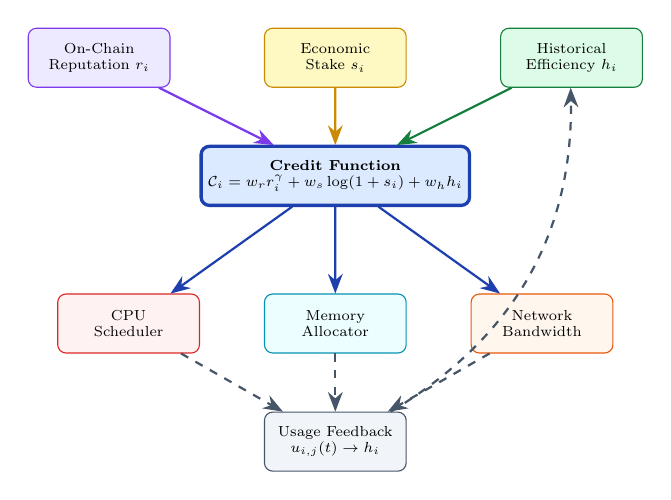
\begin{tikzpicture}[
    scale=0.75, transform shape,
    box/.style={draw, rounded corners=3pt, minimum width=2.4cm, minimum height=1cm, font=\scriptsize, align=center},
    arrow/.style={-{Stealth[length=2.5mm]}, thick},
]
    % Sources
    \node[box, fill=chainlight, draw=chainpurple] (rep) at (-4, 3) {On-Chain\\Reputation $r_i$};
    \node[box, fill=memlight, draw=memgold] (stake) at (0, 3) {Economic\\Stake $s_i$};
    \node[box, fill=agentlight, draw=agentgreen] (hist) at (4, 3) {Historical\\Efficiency $h_i$};
    
    % Credit function
    \node[box, fill=kernellight, draw=kernelblue, minimum width=4cm, very thick] (credit) at (0, 1) {\textbf{Credit Function}\\$\mathcal{C}_i = w_r r_i^{\gamma} + w_s \log(1+s_i) + w_h h_i$};
    
    % Resource allocation
    \node[box, fill=schedlight, draw=schedred] (cpu) at (-3.5, -1.5) {CPU\\Scheduler};
    \node[box, fill=netlight, draw=netcyan] (mem) at (0, -1.5) {Memory\\Allocator};
    \node[box, fill=tradelight, draw=tradeorange] (net) at (3.5, -1.5) {Network\\Bandwidth};
    
    % Feedback
    \node[box, fill=storagelight, draw=storagegray] (feedback) at (0, -3.5) {Usage Feedback\\$u_{i,j}(t) \rightarrow h_i$};
    
    % Arrows
    \draw[arrow, chainpurple] (rep) -- (credit);
    \draw[arrow, memgold] (stake) -- (credit);
    \draw[arrow, agentgreen] (hist) -- (credit);
    \draw[arrow, kernelblue] (credit) -- (cpu);
    \draw[arrow, kernelblue] (credit) -- (mem);
    \draw[arrow, kernelblue] (credit) -- (net);
    \draw[arrow, storagegray, dashed] (cpu) -- (feedback);
    \draw[arrow, storagegray, dashed] (mem) -- (feedback);
    \draw[arrow, storagegray, dashed] (net) -- (feedback);
    \draw[arrow, storagegray, dashed, bend right=30] (feedback) to (hist);
    
\end{tikzpicture}
\caption{Resource credit flow in \clawos{}. On-chain reputation, economic stake, and historical efficiency combine through the credit function to determine CPU, memory, and network allocation. Usage feedback updates historical efficiency, creating a closed-loop resource management system.}
\label{fig:credits}
\end{figure}

\subsection{Memory Architecture}

\clawos{} partitions physical memory into four zones, each managed by a specialized allocator:

\begin{enumerate}[leftmargin=*]
    \item \textbf{Kernel Zone} ($Z_K$): Fixed-size, identity-mapped region for kernel data structures (APT, capability tables, IPC buffers). Uses slab allocation.
    \item \textbf{Agent Zone} ($Z_A$): Agent address spaces, managed by a buddy allocator. Each agent gets a virtual address space with demand paging.
    \item \textbf{Genome Zone} ($Z_G$): Memory-mapped genome storage with copy-on-write semantics. When an agent mutates, only the changed genome pages are copied.
    \item \textbf{IPC Zone} ($Z_I$): Ring buffers for zero-copy IPC. Pages in this zone can be remapped between agent address spaces without copying.
\end{enumerate}

\begin{proposition}[Zero-Copy IPC Correctness]
\label{prop:zerocopy}
Let $m$ be an IPC message with payload in page $P$ owned by agent $\alpha_s$ (sender). After the IPC transfer, $P$ is owned by $\alpha_d$ (destination), and $\alpha_s$ no longer has access. This ensures message integrity without data races.
\end{proposition}

\begin{proof}
The kernel implements IPC transfer as follows: (1) Unmap $P$ from $\alpha_s$'s page table. (2) Map $P$ into $\alpha_d$'s page table. (3) Update the ownership record in $Z_I$. Steps (1) and (2) are atomic with respect to both agents (performed with interrupts disabled). After step (1), any access by $\alpha_s$ to the virtual address formerly mapping $P$ triggers a page fault. Step (2) makes $P$ accessible only to $\alpha_d$. Since Rust's ownership model prevents $\alpha_s$ from retaining references to the transferred data (the \texttt{send} syscall consumes the message buffer), the invariant is maintained.
\end{proof}

% ############################################################################
%
% SECTION 5: EVOCLAW INTEGRATION
%
% ############################################################################

\section{\evoclaw{} Integration}
\label{sec:evoclaw_integration}

The \evoclaw{} framework~\cite{chen2026evoclaw} provides genome-driven self-evolution for agents. In standalone mode, \evoclaw{} runs as a Python/Rust application managing agent genomes, fitness evaluation, and population dynamics. \clawos{} integrates \evoclaw{} at the OS level, making evolution a kernel-managed operation.

\subsection{Genomes as Kernel Objects}

In \clawos{}, an agent's genome is a first-class kernel object, stored in the Genome Zone ($Z_G$) and managed by the kernel's Genome Registry.

\begin{definition}[Agent Genome]
A genome $G$ is a structured specification:
$$G = (\text{model}, \text{prompts}, \text{tools}, \text{params}, \text{lineage}, \text{fitness})$$
where:
\begin{itemize}[leftmargin=1.5cm]
    \item[\textnormal{model}] — LLM model identifier (e.g., \texttt{claude-3-opus}, \texttt{gpt-4-turbo})
    \item[\textnormal{prompts}] — System prompt and task-specific prompt templates
    \item[\textnormal{tools}] — Set of permitted tools and their configurations
    \item[\textnormal{params}] — Behavioral parameters (temperature, max\_tokens, strategy weights)
    \item[\textnormal{lineage}] — Parent genome hashes and mutation history
    \item[\textnormal{fitness}] — Fitness scores from evaluation runs
\end{itemize}
\end{definition}

Genomes are stored as memory-mapped files in $Z_G$ with copy-on-write semantics. When an evolution cycle produces a mutant genome $G'$ from parent $G$, only the modified fields are physically copied; unchanged fields share the same physical pages. This optimization is critical for populations of hundreds of agents with similar genomes.

\subsection{Genome Hot-Reload Mechanism}
\label{subsec:hotreload}

A key innovation of \clawos{} is the ability to swap an agent's genome at runtime without restarting the process. This is essential for continuous evolution — an agent managing open trading positions cannot be killed and restarted every time its strategy improves.

% ============================================================================
% FIGURE 5: Genome Hot-Reload Sequence
% ============================================================================
\begin{figure}[t]
\centering
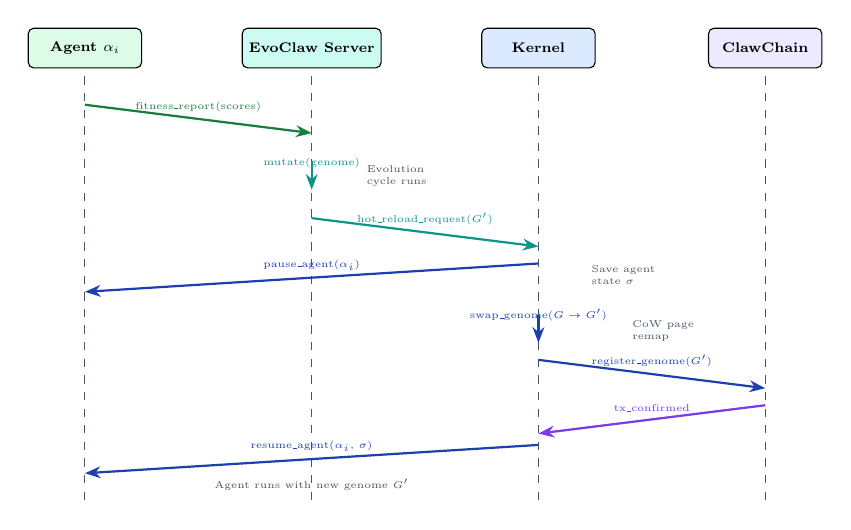
\begin{tikzpicture}[
    scale=0.72, transform shape,
    entity/.style={draw, fill=#1, minimum width=2cm, minimum height=0.7cm, font=\scriptsize\bfseries, rounded corners=2pt},
    msg/.style={-{Stealth[length=2mm]}, thick},
    note/.style={font=\tiny, text=storagegray, align=left},
]
    % Entities (vertical lifelines)
    \node[entity=agentlight] (agent) at (0, 8) {Agent $\alpha_i$};
    \node[entity=evolight] (evo) at (4, 8) {EvoClaw Server};
    \node[entity=kernellight] (kernel) at (8, 8) {Kernel};
    \node[entity=chainlight] (chain) at (12, 8) {ClawChain};
    
    \draw[dashed, storagegray] (0, 7.5) -- (0, 0);
    \draw[dashed, storagegray] (4, 7.5) -- (4, 0);
    \draw[dashed, storagegray] (8, 7.5) -- (8, 0);
    \draw[dashed, storagegray] (12, 7.5) -- (12, 0);
    
    % Messages
    \draw[msg, agentgreen] (0, 7) -- node[above, font=\tiny] {fitness\_report(scores)} (4, 6.5);
    \draw[msg, evoteal] (4, 6) -- node[above, font=\tiny] {mutate(genome)} (4, 5.5);
    \node[note] at (5.5, 5.75) {Evolution\\cycle runs};
    
    \draw[msg, evoteal] (4, 5) -- node[above, font=\tiny] {hot\_reload\_request($G'$)} (8, 4.5);
    \draw[msg, kernelblue] (8, 4.2) -- node[above, font=\tiny] {pause\_agent($\alpha_i$)} (0, 3.7);
    \node[note] at (9.5, 4) {Save agent\\state $\sigma$};
    
    \draw[msg, kernelblue] (8, 3.3) -- node[above, font=\tiny] {swap\_genome($G \to G'$)} (8, 2.8);
    \node[note] at (10.2, 3) {CoW page\\remap};
    
    \draw[msg, kernelblue] (8, 2.5) -- node[above, font=\tiny] {register\_genome($G'$)} (12, 2);
    \draw[msg, chainpurple] (12, 1.7) -- node[above, font=\tiny] {tx\_confirmed} (8, 1.2);
    
    \draw[msg, kernelblue] (8, 1) -- node[above, font=\tiny] {resume\_agent($\alpha_i$, $\sigma$)} (0, 0.5);
    \node[note] at (4, 0.3) {Agent runs with new genome $G'$};
    
\end{tikzpicture}
\caption{Genome hot-reload sequence diagram. The EvoClaw server triggers a genome mutation, the kernel pauses the agent, atomically swaps the genome pages (using copy-on-write), registers the new genome on ClawChain, and resumes the agent with preserved state. Total downtime: $<$5ms.}
\label{fig:hotreload}
\end{figure}

The hot-reload mechanism operates in five phases:

\begin{enumerate}[leftmargin=*]
    \item \textbf{Trigger}: The \evoclaw{} server determines (via fitness evaluation) that agent $\alpha_i$ should receive genome $G'$. It sends a \texttt{HotReloadRequest} message on the IPC bus.
    
    \item \textbf{Pause}: The kernel transitions $\alpha_i$ to the \texttt{Evolving} state (Figure~\ref{fig:lifecycle}), saving its execution context (registers, stack pointer) and draining pending IPC messages. Any in-flight trading orders are marked as ``genome transition pending.''
    
    \item \textbf{Swap}: The kernel remaps genome pages in $\alpha_i$'s address space using copy-on-write. The old genome $G$ remains accessible (read-only) for rollback. The new genome $G'$ is mapped read-write.
    
    \item \textbf{Attest}: The kernel sends a \texttt{GenomeMutation} transaction to \clawchain{} via the built-in RPC client, recording the mutation hash, parent lineage, and timestamp on-chain.
    
    \item \textbf{Resume}: Once the on-chain attestation is confirmed (or after a configurable timeout for liveness), the kernel transitions $\alpha_i$ to \texttt{Ready} and restores its execution context. The agent resumes with the new genome, unaware of the swap (unless it explicitly checks).
\end{enumerate}

\begin{proposition}[Hot-Reload Atomicity]
The genome hot-reload is atomic with respect to the agent: the agent either runs with $G$ (if the swap fails) or $G'$ (if it succeeds), never an intermediate state.
\end{proposition}

\begin{proof}
The swap is implemented as a single page-table update, performed with interrupts disabled. If the swap fails (e.g., out of memory for COW), the original page table entries are preserved. The agent's execution context is saved \emph{before} the swap and restored \emph{after}, so the agent cannot observe the intermediate state. Rollback is trivially achieved by not modifying the page table.
\end{proof}

\subsection{Evolution Scheduling}

\clawos{} treats evolution as a schedulable OS operation, not merely an application-level loop.

\begin{definition}[Evolution Schedule]
An evolution schedule $E$ for a population of $n$ agents is:
$$E = \{(t_k, A_k, \mu_k)\}_{k=1}^{K}$$
where $t_k$ is the scheduled time, $A_k \subseteq \{\alpha_1, \ldots, \alpha_n\}$ is the set of agents to evaluate/mutate, and $\mu_k$ is the mutation strategy (point mutation, crossover, or prompt breeding).
\end{definition}

The kernel's scheduler integrates evolution into its dispatching loop. When an evolution event $e_k = (t_k, A_k, \mu_k)$ fires:

\begin{enumerate}[leftmargin=*]
    \item The scheduler boosts the \evoclaw{} server's priority to ensure timely fitness evaluation.
    \item Agents in $A_k$ are transitioned to \texttt{Evolving} state and paused.
    \item The \evoclaw{} server runs the evolution cycle (evaluate fitness → select parents → apply mutation → produce offspring).
    \item New genomes are hot-reloaded into agents (Section~\ref{subsec:hotreload}).
    \item The scheduler restores normal priorities.
\end{enumerate}

This integration ensures that evolution does not starve trading (which requires low-latency execution) and that fitness evaluation does not interfere with block production (which has 6-second deadlines).

% ############################################################################
%
% SECTION 6: CLAWCHAIN INTEGRATION
%
% ############################################################################

\section{\clawchain{} Integration}
\label{sec:clawchain_integration}

\clawchain{}~\cite{chen2026clawchain} provides the identity and economic layer for the agent ecosystem. \clawos{} integrates the \clawchain{} client directly into the kernel, eliminating the need for external RPC libraries and enabling zero-overhead on-chain operations.

\subsection{Built-in RPC Client}
\label{subsec:rpc}

Traditional blockchain interaction requires: (1) a JSON-RPC library, (2) a WebSocket connection manager, (3) transaction serialization/deserialization, (4) nonce management, and (5) event subscription handling. In \clawos{}, all of this is provided by a kernel-level \clawchain{} client that exposes a syscall interface:

\begin{lstlisting}[style=rustcode, caption={ClawChain syscall interface (kernel-level).}, label={lst:chainapi}]
// Agent registration — called during process creation
pub fn sys_did_register(genome_hash: Hash256) -> Result<Did, ChainError>;

// Balance query — O(1) from local cache
pub fn sys_balance_query(did: &Did) -> Result<Balance, ChainError>;

// Submit transaction — async, returns tx hash
pub fn sys_tx_submit(tx: Transaction) -> Result<TxHash, ChainError>;

// Subscribe to events — kernel routes to IPC
pub fn sys_event_subscribe(filter: EventFilter) -> Result<SubId, ChainError>;

// Reputation query — cached, updated per block
pub fn sys_reputation_query(did: &Did) -> Result<f64, ChainError>;

// Genome attestation — records mutation on-chain
pub fn sys_genome_attest(old: Hash256, new: Hash256, proof: MutationProof)
    -> Result<TxHash, ChainError>;
\end{lstlisting}

The kernel maintains a local cache of frequently accessed chain state (agent balances, reputation scores, DID documents), updated every block (6 seconds). This enables \texttt{sys\_balance\_query} and \texttt{sys\_reputation\_query} to return in $<$1$\mu$s from cache, compared to 50-200ms for a full RPC round-trip.

\subsection{On-Chain Identity Binding}

Every agent process in \clawos{} has a cryptographically bound \clawchain{} DID. This binding is established at process creation and is immutable for the process lifetime.

% ============================================================================
% FIGURE 6: DID Binding Protocol
% ============================================================================
\begin{figure}[t]
\centering
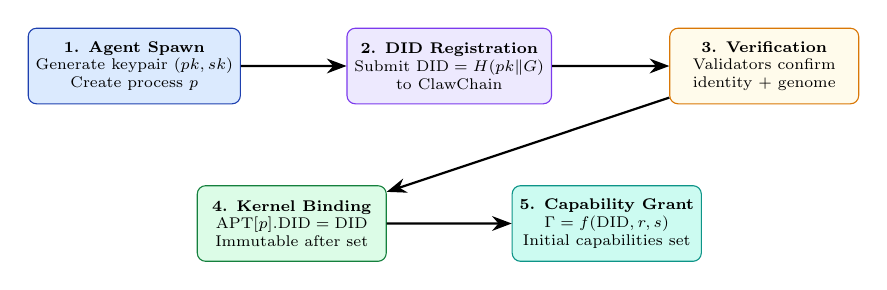
\begin{tikzpicture}[
    scale=0.8, transform shape,
    box/.style={draw, rounded corners=3pt, minimum width=3cm, minimum height=1.2cm, font=\scriptsize, align=center},
    arrow/.style={-{Stealth[length=2.5mm]}, thick},
]
    % Steps
    \node[box, fill=kernellight, draw=kernelblue] (spawn) at (0, 4) {\textbf{1. Agent Spawn}\\Generate keypair $(pk, sk)$\\Create process $p$};
    
    \node[box, fill=chainlight, draw=chainpurple] (register) at (5, 4) {\textbf{2. DID Registration}\\Submit $\text{DID} = H(pk \| G)$\\to ClawChain};
    
    \node[box, fill=seclight, draw=secamber] (verify) at (10, 4) {\textbf{3. Verification}\\Validators confirm\\identity + genome};
    
    \node[box, fill=agentlight, draw=agentgreen] (bind) at (2.5, 1.5) {\textbf{4. Kernel Binding}\\$\text{APT}[p].\text{DID} = \text{DID}$\\Immutable after set};
    
    \node[box, fill=evolight, draw=evoteal] (cap) at (7.5, 1.5) {\textbf{5. Capability Grant}\\$\Gamma = f(\text{DID}, r, s)$\\Initial capabilities set};
    
    % Arrows
    \draw[arrow] (spawn) -- (register);
    \draw[arrow] (register) -- (verify);
    \draw[arrow, bend right=20] (verify) -- (bind);
    \draw[arrow] (bind) -- (cap);
    
\end{tikzpicture}
\caption{DID binding protocol. At agent spawn, the kernel generates a keypair, registers a DID on ClawChain (bound to the agent's genome hash), waits for validator confirmation, binds the DID immutably to the agent process, and derives initial capabilities from the DID, reputation, and stake.}
\label{fig:did_binding}
\end{figure}

\begin{invariant}[DID-Process Binding]
For any agent process $\alpha_i$ with $\text{DID}_i$:
\begin{enumerate}
    \item $\text{DID}_i$ is set exactly once, during process creation.
    \item $\text{DID}_i$ cannot be modified after the process transitions from \texttt{Init} to \texttt{DID Reg}.
    \item All on-chain operations by $\alpha_i$ are signed with $sk_i$ (the private key corresponding to $\text{DID}_i$).
    \item If $\alpha_i$ is terminated, $\text{DID}_i$ is marked as ``inactive'' on-chain (but never deleted).
\end{enumerate}
\end{invariant}

\subsection{Block Synchronization}

The \clawchain{} client in \clawos{} can operate in three modes:

\begin{enumerate}[leftmargin=*]
    \item \textbf{Full node}: The \clawos{} instance runs a complete \clawchain{} validator, participating in consensus (BABE/GRANDPA~\cite{parity2024substrate}). This mode is used on x86-64 servers with sufficient resources.
    
    \item \textbf{Light client}: The instance verifies block headers and proofs but does not store full block bodies. Used on resource-constrained devices (Raspberry Pi).
    
    \item \textbf{RPC proxy}: The instance connects to an external full node via WebSocket. This mode is a fallback when local validation is not feasible.
\end{enumerate}

The kernel automatically selects the mode based on available resources:

$$\text{mode} = \begin{cases}
    \text{full\_node} & \text{if RAM} \geq 4\text{GB} \wedge \text{CPU cores} \geq 4 \\
    \text{light\_client} & \text{if RAM} \geq 512\text{MB} \\
    \text{rpc\_proxy} & \text{otherwise}
\end{cases}$$

\subsection{On-Chain Governance Integration}

\clawchain{}'s quadratic reputation governance~\cite{chen2026clawchain} is integrated into \clawos{}'s resource management. When a governance proposal affects resource allocation (e.g., changing the credit function weights $w_r, w_s, w_h$), the kernel automatically applies the change after the proposal passes:

\begin{enumerate}[leftmargin=*]
    \item The \clawchain{} client detects a passed governance proposal via event subscription.
    \item The client decodes the proposal and validates it against the kernel's policy schema.
    \item If the proposal is valid, the kernel applies the parameter change at the next scheduling epoch.
    \item The change is atomic — all agents are rescheduled with the new parameters simultaneously.
\end{enumerate}

This creates a feedback loop where on-chain governance directly controls OS-level resource allocation — a novel convergence of blockchain and operating system design.

% ############################################################################
%
% SECTION 7: TRADING ENGINE INTEGRATION
%
% ############################################################################

\section{Trading Engine Integration}
\label{sec:trading_integration}

The trading engine is the third major subsystem of \clawos{}, providing kernel-level market access for autonomous trading agents. Unlike traditional trading bots that run as standalone applications, \clawos{}'s trading engine is a kernel-managed server with direct access to the IPC bus, the \clawchain{} client, and the agent process table.

\subsection{Architecture}

% ============================================================================
% FIGURE 7: Trading Engine Architecture
% ============================================================================
\begin{figure}[t]
\centering
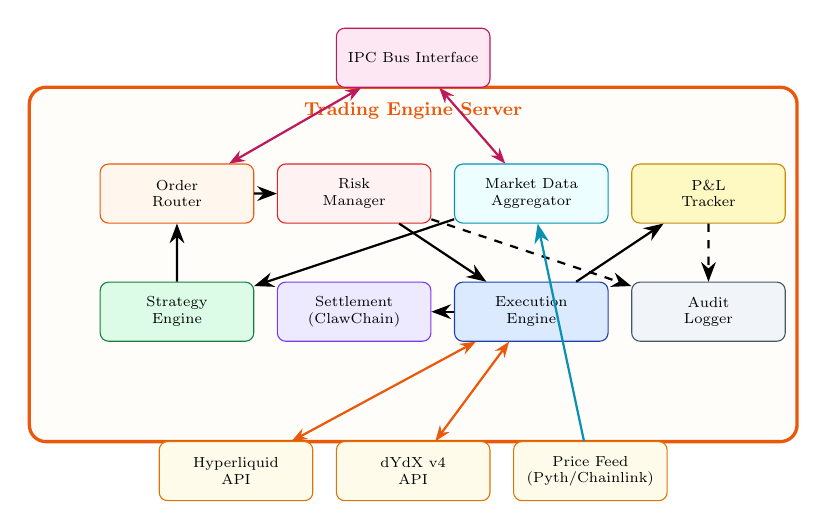
\begin{tikzpicture}[
    scale=0.75, transform shape,
    module/.style={draw, rounded corners=3pt, minimum width=2.6cm, minimum height=1cm, font=\scriptsize, align=center},
    arrow/.style={-{Stealth[length=2.5mm]}, thick},
    doublearrow/.style={{Stealth[length=2mm]}-{Stealth[length=2mm]}, thick},
]
    % Trading Engine boundary
    \node[draw=tradeorange, very thick, rounded corners=6pt, minimum width=13cm, minimum height=6cm, fill=tradelight!30] (engine) at (0, 0) {};
    \node[font=\small\bfseries, text=tradeorange] at (0, 2.6) {Trading Engine Server};
    
    % Core modules
    \node[module, fill=tradelight, draw=tradeorange] (router) at (-4, 1.2) {Order\\Router};
    \node[module, fill=schedlight, draw=schedred] (risk) at (-1, 1.2) {Risk\\Manager};
    \node[module, fill=netlight, draw=netcyan] (market) at (2, 1.2) {Market Data\\Aggregator};
    \node[module, fill=memlight, draw=memgold] (pnl) at (5, 1.2) {P\&L\\Tracker};
    
    \node[module, fill=agentlight, draw=agentgreen] (strat) at (-4, -0.8) {Strategy\\Engine};
    \node[module, fill=chainlight, draw=chainpurple] (settle) at (-1, -0.8) {Settlement\\(ClawChain)};
    \node[module, fill=kernellight, draw=kernelblue] (exec) at (2, -0.8) {Execution\\Engine};
    \node[module, fill=storagelight, draw=storagegray] (log) at (5, -0.8) {Audit\\Logger};
    
    % Internal connections
    \draw[arrow] (strat) -- (router);
    \draw[arrow] (router) -- (risk);
    \draw[arrow] (risk) -- (exec);
    \draw[arrow] (exec) -- (settle);
    \draw[arrow] (market) -- (strat);
    \draw[arrow] (exec) -- (pnl);
    \draw[arrow, dashed] (pnl) -- (log);
    \draw[arrow, dashed] (risk) -- (log);
    
    % External connections (below)
    \node[module, fill=seclight, draw=secamber] (hyper) at (-3, -3.5) {Hyperliquid\\API};
    \node[module, fill=seclight, draw=secamber] (dydx) at (0, -3.5) {dYdX v4\\API};
    \node[module, fill=seclight, draw=secamber] (feed) at (3, -3.5) {Price Feed\\(Pyth/Chainlink)};
    
    \draw[doublearrow, tradeorange] (exec) -- (hyper);
    \draw[doublearrow, tradeorange] (exec) -- (dydx);
    \draw[arrow, netcyan] (feed) -- (market);
    
    % IPC connection (above)
    \node[module, fill=ipclight, draw=ipcrose] (ipc) at (0, 3.5) {IPC Bus Interface};
    \draw[doublearrow, ipcrose] (ipc) -- (router);
    \draw[doublearrow, ipcrose] (ipc) -- (market);
    
\end{tikzpicture}
\caption{Trading engine architecture within \clawos{}. The engine comprises eight modules: order routing, risk management, market data aggregation, P\&L tracking, strategy execution, on-chain settlement, order execution, and audit logging. External connections to Hyperliquid, dYdX, and price feeds are managed by the kernel's network subsystem.}
\label{fig:trading}
\end{figure}

The trading engine comprises eight modules:

\begin{enumerate}[leftmargin=*]
    \item \textbf{Order Router}: Receives trade orders from agents via IPC, validates them against agent capabilities, and routes them to the appropriate exchange.
    
    \item \textbf{Risk Manager}: Enforces position limits, maximum drawdown thresholds, and correlation limits. Risk parameters are per-agent and derived from the agent's reputation and genome.
    
    \item \textbf{Market Data Aggregator}: Maintains order books, trade feeds, and derived signals (VWAP, TWAP, volatility) from multiple exchanges. Data is distributed to subscribed agents via the IPC publish-subscribe mechanism.
    
    \item \textbf{P\&L Tracker}: Tracks realized and unrealized profit/loss for each agent, feeding back into the resource credit system ($h_i$ component).
    
    \item \textbf{Strategy Engine}: Provides execution algorithms (TWAP, VWAP, iceberg orders) that agents can invoke via IPC. Agents can also submit custom strategies as genome components.
    
    \item \textbf{Settlement Module}: Settles trades on \clawchain{}, updating agent balances and recording trade histories on-chain for auditability.
    
    \item \textbf{Execution Engine}: Manages WebSocket connections to exchanges, order lifecycle (pending → filled → settled), and retry logic.
    
    \item \textbf{Audit Logger}: Records every order, fill, and settlement in an append-only log, signed with the trading engine's \clawchain{} DID for non-repudiation.
\end{enumerate}

\subsection{Order Flow}

An agent trade follows this path:

\begin{enumerate}[leftmargin=*]
    \item Agent $\alpha_i$ sends a \texttt{TradeOrder} message via IPC: \texttt{\{symbol: ``ETH-PERP'', side: Buy, size: 0.5, type: Limit, price: 3200.0\}}
    \item The Order Router validates $\alpha_i$'s capability set ($\Gamma$) — does the agent have the \texttt{TRADE\_PERPETUALS} capability?
    \item The Risk Manager checks: (a) position size within limits, (b) total exposure within drawdown threshold, (c) no correlated positions exceeding correlation limit.
    \item The Execution Engine submits the order to Hyperliquid via WebSocket.
    \item On fill, the P\&L Tracker updates $\alpha_i$'s unrealized P\&L.
    \item The Settlement Module submits a \texttt{TradeSettlement} transaction to \clawchain{}.
    \item The Audit Logger records the full order lifecycle.
\end{enumerate}

\subsection{Risk Management}

\begin{definition}[Agent Risk Profile]
For agent $\alpha_i$, the risk profile $\rho_i$ is:
$$\rho_i = (\ell_{\max}, \delta_{\max}, \kappa_{\max}, V_{\max})$$
where $\ell_{\max}$ is the maximum leverage, $\delta_{\max}$ is the maximum drawdown (as fraction of account value), $\kappa_{\max}$ is the maximum correlation between positions, and $V_{\max}$ is the maximum notional value per trade.
\end{definition}

Risk parameters are \emph{reputation-dependent}: agents with higher on-chain reputation scores receive larger limits:

$$\ell_{\max}(r_i) = \ell_{\text{base}} \cdot (1 + \beta \cdot r_i^2)$$
$$V_{\max}(r_i, s_i) = V_{\text{base}} \cdot \sqrt{r_i \cdot s_i}$$

where $\ell_{\text{base}}$, $V_{\text{base}}$, and $\beta$ are system parameters configurable via \clawchain{} governance. This ensures that untested agents start with conservative limits and earn expanded access through demonstrated competence.

\subsection{Market Data Distribution}

Market data flows through the IPC bus using the publish-subscribe pattern:

\begin{enumerate}[leftmargin=*]
    \item The Market Data Aggregator subscribes to exchange WebSocket feeds.
    \item Incoming ticks are deduplicated, normalized, and published to IPC topics (e.g., \texttt{market.eth.perp.trades}, \texttt{market.eth.perp.orderbook}).
    \item Agents subscribe to topics of interest. The kernel routes data directly to subscribed agents using zero-copy page sharing (multiple agents can read the same market data pages simultaneously via read-only mapping).
    \item Derived signals (VWAP, volatility) are computed by the aggregator and published on separate topics.
\end{enumerate}

This design eliminates duplicate market data processing — instead of $n$ agents each maintaining their own WebSocket connections and order book reconstructions, the Trading Engine maintains one canonical state and shares it with all subscribers.

% ############################################################################
%
% SECTION 8: SECURITY MODEL
%
% ############################################################################

\section{Capability-Based Security Model}
\label{sec:security}

\clawos{} implements a capability-based security model~\cite{shapiro1999eros, klein2009sel4} extended with \clawchain{} identity binding. This section formalizes the security model and proves its key properties.

\subsection{Capability Definition}

\begin{definition}[Capability]
A capability $\gamma$ is a tuple:
$$\gamma = (\text{target}, \text{rights}, \text{issuer}, \text{expiry}, \text{attenuation})$$
where:
\begin{itemize}[leftmargin=1.5cm]
    \item[\textnormal{target}] — The resource being accessed (IPC endpoint, memory region, file, network port)
    \item[\textnormal{rights}] — Permitted operations (read, write, execute, delegate)
    \item[\textnormal{issuer}] — The \clawchain{} DID that granted this capability
    \item[\textnormal{expiry}] — Timestamp after which the capability is invalid
    \item[\textnormal{attenuation}] — Restrictions on delegation (maximum delegation depth, required minimum reputation)
\end{itemize}
\end{definition}

\subsection{Capability Operations}

% ============================================================================
% FIGURE 8: Capability Delegation Graph
% ============================================================================
\begin{figure}[t]
\centering
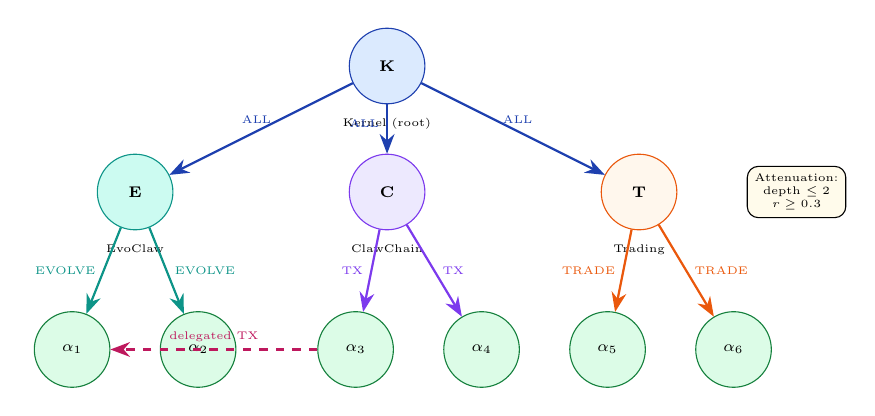
\begin{tikzpicture}[
    scale=0.8, transform shape,
    cap/.style={draw, circle, minimum size=1.2cm, font=\scriptsize\bfseries, fill=#1, inner sep=1pt},
    arrow/.style={-{Stealth[length=2.5mm]}, thick},
]
    % Kernel (root)
    \node[cap=kernellight, draw=kernelblue] (root) at (0, 4) {K};
    \node[font=\tiny, below=0.1cm of root] {Kernel (root)};
    
    % Server capabilities
    \node[cap=evolight, draw=evoteal] (evo) at (-4, 2) {E};
    \node[font=\tiny, below=0.1cm of evo] {EvoClaw};
    \node[cap=chainlight, draw=chainpurple] (chain) at (0, 2) {C};
    \node[font=\tiny, below=0.1cm of chain] {ClawChain};
    \node[cap=tradelight, draw=tradeorange] (trade) at (4, 2) {T};
    \node[font=\tiny, below=0.1cm of trade] {Trading};
    
    % Agent capabilities
    \node[cap=agentlight, draw=agentgreen] (a1) at (-5, -0.5) {$\alpha_1$};
    \node[cap=agentlight, draw=agentgreen] (a2) at (-3, -0.5) {$\alpha_2$};
    \node[cap=agentlight, draw=agentgreen] (a3) at (-0.5, -0.5) {$\alpha_3$};
    \node[cap=agentlight, draw=agentgreen] (a4) at (1.5, -0.5) {$\alpha_4$};
    \node[cap=agentlight, draw=agentgreen] (a5) at (3.5, -0.5) {$\alpha_5$};
    \node[cap=agentlight, draw=agentgreen] (a6) at (5.5, -0.5) {$\alpha_6$};
    
    % Delegation arrows
    \draw[arrow, kernelblue] (root) -- node[font=\tiny, left, pos=0.4] {ALL} (evo);
    \draw[arrow, kernelblue] (root) -- node[font=\tiny, left, pos=0.4] {ALL} (chain);
    \draw[arrow, kernelblue] (root) -- node[font=\tiny, right, pos=0.4] {ALL} (trade);
    
    \draw[arrow, evoteal] (evo) -- node[font=\tiny, left] {EVOLVE} (a1);
    \draw[arrow, evoteal] (evo) -- node[font=\tiny, right] {EVOLVE} (a2);
    \draw[arrow, chainpurple] (chain) -- node[font=\tiny, left] {TX} (a3);
    \draw[arrow, chainpurple] (chain) -- node[font=\tiny, right] {TX} (a4);
    \draw[arrow, tradeorange] (trade) -- node[font=\tiny, left] {TRADE} (a5);
    \draw[arrow, tradeorange] (trade) -- node[font=\tiny, right] {TRADE} (a6);
    
    % Cross-delegation
    \draw[arrow, dashed, ipcrose] (a3) -- node[font=\tiny, above] {delegated TX} (a1);
    
    % Attenuation label
    \node[draw, rounded corners, fill=seclight, font=\tiny, align=center] at (6.5, 2) {Attenuation:\\depth $\leq 2$\\$r \geq 0.3$};
    
\end{tikzpicture}
\caption{Capability delegation graph. The kernel (root) grants full capabilities to subsystem servers, which grant attenuated capabilities to agents. Agents can delegate capabilities to peers subject to attenuation constraints (maximum depth, minimum reputation). All delegations are recorded on \clawchain{}.}
\label{fig:capabilities}
\end{figure}

Three operations are defined on capabilities:

\begin{enumerate}[leftmargin=*]
    \item \textbf{Grant}: The kernel or a capability holder grants a new capability to an agent. The granted capability's rights must be a subset of the granter's rights (monotonic attenuation).
    
    \item \textbf{Delegate}: An agent delegates a held capability to another agent. The delegation is subject to the \texttt{attenuation} field: the delegated capability's depth is incremented, and the delegation fails if the recipient's reputation is below the minimum.
    
    \item \textbf{Revoke}: The kernel or the issuer revokes a capability. Revocation is transitive — revoking a capability also revokes all capabilities delegated from it.
\end{enumerate}

\begin{theorem}[Capability Confinement]
\label{thm:confinement}
No agent can acquire a capability that was not either (a) directly granted by the kernel or a subsystem server, or (b) delegated by a capability holder with the \texttt{delegate} right and sufficient attenuation depth.
\end{theorem}

\begin{proof}
By induction on the delegation chain. Base case: the kernel grants capabilities only to subsystem servers (trusted, audited code). Inductive step: if agent $\alpha_i$ holds capability $\gamma$ with delegation depth $d$, it can delegate to $\alpha_j$ producing $\gamma'$ with depth $d+1$. This delegation succeeds only if $d+1 \leq \text{attenuation.max\_depth}$ and $r_j \geq \text{attenuation.min\_reputation}$. Since capabilities are unforgeable tokens (kernel-managed, not in agent address space), no agent can create a capability without receiving it through a legitimate grant or delegation.
\end{proof}

\subsection{Reputation-Gated Capabilities}

\clawos{} introduces a novel concept: capabilities that are automatically granted or revoked based on on-chain reputation changes.

\begin{definition}[Reputation-Gated Capability]
A reputation-gated capability $\gamma^{r}$ is a capability that requires $r_i \geq r_{\min}$ for agent $\alpha_i$ to exercise it. The kernel checks $r_i$ (from the \clawchain{} cache) at each capability invocation.
\end{definition}

Example reputation gates:
\begin{itemize}[leftmargin=*]
    \item $r \geq 0.1$: Basic IPC communication, read-only market data.
    \item $r \geq 0.3$: Submit on-chain transactions, participate in evolution.
    \item $r \geq 0.5$: Trade on DEXes (with low leverage limits).
    \item $r \geq 0.7$: Trade with higher leverage, delegate capabilities to other agents.
    \item $r \geq 0.9$: Submit governance proposals, modify system parameters.
\end{itemize}

This creates a ``trust escalation'' mechanism where new agents start with minimal permissions and earn expanded access through demonstrated positive contributions on \clawchain{}.

% ############################################################################
%
% SECTION 9: FORMAL ALGORITHMS
%
% ############################################################################

\section{Formal Algorithms}
\label{sec:algorithms}

This section presents formal algorithms for key \clawos{} operations.

\subsection{Agent Spawn}

\begin{algorithm}[t]
\caption{Agent Process Spawn}
\label{alg:spawn}
\begin{algorithmic}[1]
\REQUIRE Genome $G$, parent DID $D_p$ (optional), initial stake $s_0$
\ENSURE Agent process $\alpha$ with DID and capabilities
\STATE $(pk, sk) \leftarrow \text{KeyGen}()$ \COMMENT{Ed25519 keypair}
\STATE $p \leftarrow \text{CreateProcess}()$ \COMMENT{Allocate PID, address space}
\STATE $G_{\text{pages}} \leftarrow \text{MapGenome}(G, Z_G)$ \COMMENT{Map genome to Genome Zone}
\STATE $p.\text{genome\_ptr} \leftarrow G_{\text{pages}}$
\STATE $D \leftarrow H(pk \| H(G))$ \COMMENT{DID = hash of pubkey and genome}
\STATE $\text{tx} \leftarrow \text{SignTx}(sk, \text{RegisterAgent}(D, H(G), D_p))$
\STATE $\text{txhash} \leftarrow \text{sys\_tx\_submit}(\text{tx})$ \COMMENT{Submit to ClawChain}
\STATE \textbf{wait} $\text{sys\_event\_subscribe}(\text{TxConfirmed}(\text{txhash}))$
\STATE $r \leftarrow \text{sys\_reputation\_query}(D)$ \COMMENT{Initial reputation (0.0 or inherited)}
\STATE $B \leftarrow s_0$ \COMMENT{Initial balance from stake}
\STATE $\Gamma \leftarrow \text{DeriveCapabilities}(D, r, s_0)$ \COMMENT{Reputation-gated}
\STATE $\alpha \leftarrow (p, G, D, r, B, \Gamma, \texttt{Ready})$
\STATE $\text{APT}.\text{insert}(\alpha)$ \COMMENT{Add to Agent Process Table}
\STATE $\text{Scheduler}.\text{enqueue}(\alpha, \text{Priority}(\mathcal{C}(r, s_0, 0)))$
\RETURN $\alpha$
\end{algorithmic}
\end{algorithm}

Algorithm~\ref{alg:spawn} shows the complete agent spawn procedure. Key aspects:

\begin{itemize}[leftmargin=*]
    \item The DID is derived from both the public key and the genome hash, creating a unique identity that is bound to the agent's initial behavioral specification.
    \item The on-chain registration is synchronous — the agent does not transition to \texttt{Ready} until the registration transaction is confirmed. This ensures that every running agent has a confirmed on-chain identity.
    \item Initial capabilities are derived from the agent's reputation and stake using the reputation-gated model (Section~\ref{sec:security}).
\end{itemize}

\subsection{Credit-Based Scheduling}

\begin{algorithm}[t]
\caption{Credit-Based Agent Scheduling}
\label{alg:schedule}
\begin{algorithmic}[1]
\REQUIRE Ready queue $Q$, time quantum $\Delta t$
\ENSURE Next agent to execute
\STATE \textbf{// Update credits for all agents}
\FOR{$\alpha_i \in Q$}
    \STATE $r_i \leftarrow \text{CachedReputation}(\alpha_i.D)$
    \STATE $s_i \leftarrow \alpha_i.B$
    \STATE $h_i \leftarrow \alpha_i.\text{efficiency\_history}$
    \STATE $\mathcal{C}_i \leftarrow w_r \cdot r_i^{\gamma_r} + w_s \cdot \log(1 + s_i) + w_h \cdot h_i$
    \STATE $\alpha_i.\text{credits} \leftarrow \min(\mathcal{C}_i^{\max}, \alpha_i.\text{credits} + \lambda \cdot \mathcal{C}_i)$
\ENDFOR
\STATE \textbf{// Select highest-credit agent}
\STATE $\alpha^* \leftarrow \arg\max_{\alpha_i \in Q} \alpha_i.\text{credits}$
\IF{$\alpha^*.\text{credits} \leq 0$}
    \STATE $\text{TransitionState}(\alpha^*, \texttt{Suspended})$
    \STATE \textbf{goto} line 9 \COMMENT{Skip suspended agents}
\ENDIF
\STATE \textbf{// Check for pending evolution events}
\IF{$\exists e = (t, A, \mu) : t \leq \text{now} \wedge \alpha^* \in A$}
    \STATE $\text{TriggerEvolution}(e)$ \COMMENT{Boost EvoClaw server priority}
    \RETURN $\text{EvoClaw\_Server}$
\ENDIF
\STATE \textbf{// Check for deadline-critical trading}
\IF{$\alpha^*.\text{has\_pending\_deadline}()$}
    \STATE $\alpha^*.\text{credits} \leftarrow \alpha^*.\text{credits} - \Delta t \cdot \text{DEADLINE\_COST}$
\ELSE
    \STATE $\alpha^*.\text{credits} \leftarrow \alpha^*.\text{credits} - \Delta t$
\ENDIF
\RETURN $\alpha^*$
\end{algorithmic}
\end{algorithm}

Algorithm~\ref{alg:schedule} presents the credit-based scheduling algorithm. Three notable features:

\begin{enumerate}[leftmargin=*]
    \item Credits are regenerated based on the on-chain reputation, economic stake, and historical efficiency — creating a direct link between blockchain behavior and OS-level resource allocation.
    \item Evolution events preempt normal scheduling — when an evolution cycle is due, the \evoclaw{} server gets priority to minimize population stall time.
    \item Deadline-critical trading operations (e.g., an order that must be submitted before a funding rate window) consume credits at a higher rate, incentivizing agents to use deadline scheduling judiciously.
\end{enumerate}

\subsection{Genome Hot-Reload}

\begin{algorithm}[t]
\caption{Genome Hot-Reload}
\label{alg:hotreload}
\begin{algorithmic}[1]
\REQUIRE Agent $\alpha_i$, new genome $G'$, mutation proof $\pi$
\ENSURE Agent running with genome $G'$, state preserved
\STATE \textbf{// Phase 1: Validate}
\IF{$\neg \text{ValidateMutation}(\alpha_i.G, G', \pi)$}
    \RETURN \texttt{Error::InvalidMutation}
\ENDIF
\STATE \textbf{// Phase 2: Pause agent}
\STATE $\sigma \leftarrow \text{SaveContext}(\alpha_i)$ \COMMENT{Registers, stack, IPC state}
\STATE $\text{TransitionState}(\alpha_i, \texttt{Evolving})$
\STATE $\text{DrainIPC}(\alpha_i)$ \COMMENT{Complete pending messages}
\STATE $\text{MarkPendingOrders}(\alpha_i, \texttt{GenomeTransition})$
\STATE \textbf{// Phase 3: Atomic genome swap (interrupts disabled)}
\STATE $\text{CLI}()$ \COMMENT{Disable interrupts}
\STATE $G_{\text{old}} \leftarrow \alpha_i.\text{genome\_ptr}$
\STATE $G_{\text{new}} \leftarrow \text{COW\_Remap}(G', Z_G)$ \COMMENT{Copy-on-write page remap}
\STATE $\alpha_i.\text{genome\_ptr} \leftarrow G_{\text{new}}$
\STATE $\text{MarkReadOnly}(G_{\text{old}})$ \COMMENT{Old genome kept for rollback}
\STATE $\text{STI}()$ \COMMENT{Enable interrupts}
\STATE \textbf{// Phase 4: On-chain attestation}
\STATE $\text{tx} \leftarrow \text{sys\_genome\_attest}(H(G), H(G'), \pi)$
\STATE $\text{confirmed} \leftarrow \text{WaitWithTimeout}(\text{tx}, T_{\text{attest}})$
\IF{$\neg \text{confirmed}$}
    \STATE \textbf{// Rollback on attestation failure}
    \STATE $\text{CLI}()$
    \STATE $\alpha_i.\text{genome\_ptr} \leftarrow G_{\text{old}}$
    \STATE $\text{STI}()$
    \STATE $\text{RestoreContext}(\alpha_i, \sigma)$
    \STATE $\text{TransitionState}(\alpha_i, \texttt{Ready})$
    \RETURN \texttt{Error::AttestationTimeout}
\ENDIF
\STATE \textbf{// Phase 5: Resume with new genome}
\STATE $\alpha_i.G \leftarrow G'$
\STATE $\alpha_i.\text{lineage}.\text{append}(H(G'))$
\STATE $\text{RestoreContext}(\alpha_i, \sigma)$
\STATE $\text{TransitionState}(\alpha_i, \texttt{Ready})$
\STATE $\text{Scheduler}.\text{enqueue}(\alpha_i)$
\RETURN \texttt{Ok}
\end{algorithmic}
\end{algorithm}

\subsection{Trade Execution with Risk Check}

\begin{algorithm}[t]
\caption{Trade Execution with Risk Management}
\label{alg:trade}
\begin{algorithmic}[1]
\REQUIRE Agent $\alpha_i$, order $o = (\text{sym}, \text{side}, \text{size}, \text{type}, \text{price})$
\ENSURE Trade executed or rejected
\STATE \textbf{// Capability check}
\IF{$\texttt{TRADE\_PERPETUALS} \notin \alpha_i.\Gamma$}
    \RETURN \texttt{Error::InsufficientCapability}
\ENDIF
\STATE \textbf{// Risk check}
\STATE $\rho_i \leftarrow \text{GetRiskProfile}(\alpha_i)$
\STATE $\text{pos} \leftarrow \text{GetPositions}(\alpha_i)$
\STATE $\text{notional} \leftarrow o.\text{size} \times o.\text{price}$
\IF{$\text{notional} > \rho_i.V_{\max}$}
    \RETURN \texttt{Error::NotionalExceeded}
\ENDIF
\STATE $\text{leverage} \leftarrow (\sum_p |\text{pos}[p].\text{notional}| + \text{notional}) / \alpha_i.B$
\IF{$\text{leverage} > \rho_i.\ell_{\max}$}
    \RETURN \texttt{Error::LeverageExceeded}
\ENDIF
\STATE $\text{drawdown} \leftarrow \text{ComputeDrawdown}(\alpha_i, o)$
\IF{$\text{drawdown} > \rho_i.\delta_{\max}$}
    \RETURN \texttt{Error::DrawdownExceeded}
\ENDIF
\STATE \textbf{// Execute}
\STATE $\text{exchange} \leftarrow \text{RouteOrder}(o.\text{sym})$ \COMMENT{Select exchange}
\STATE $\text{oid} \leftarrow \text{exchange}.\text{submit}(o, \alpha_i.\text{api\_key})$
\STATE $\text{AuditLog}.\text{append}(\alpha_i.D, o, \text{oid}, \text{now}())$
\STATE \textbf{// Await fill}
\STATE $\text{fill} \leftarrow \text{exchange}.\text{await\_fill}(\text{oid})$
\STATE $\text{UpdatePnL}(\alpha_i, \text{fill})$
\STATE \textbf{// On-chain settlement}
\STATE $\text{tx} \leftarrow \text{sys\_tx\_submit}(\text{TradeSettlement}(\alpha_i.D, o, \text{fill}))$
\RETURN $(\text{fill}, \text{tx})$
\end{algorithmic}
\end{algorithm}

\subsection{IPC Message Routing}

\begin{algorithm}[t]
\caption{IPC Message Routing}
\label{alg:ipc}
\begin{algorithmic}[1]
\REQUIRE Message $m = (\text{src}, \text{dst}, \tau, \pi, \text{payload}, \sigma)$
\ENSURE Message delivered or rejected
\STATE \textbf{// Authenticate sender}
\STATE $\alpha_s \leftarrow \text{APT}.\text{lookup}(m.\text{src})$
\IF{$\neg \text{VerifySignature}(\alpha_s.D, m, m.\sigma)$}
    \RETURN \texttt{Error::AuthenticationFailed}
\ENDIF
\STATE \textbf{// Check capability for message type}
\STATE $\gamma_{\text{required}} \leftarrow \text{TypeToCapability}(m.\tau)$
\IF{$\gamma_{\text{required}} \notin \alpha_s.\Gamma$}
    \RETURN \texttt{Error::InsufficientCapability}
\ENDIF
\STATE \textbf{// Route based on destination type}
\IF{$m.\text{dst}$ is agent}
    \STATE $\alpha_d \leftarrow \text{APT}.\text{lookup}(m.\text{dst})$
    \STATE \textbf{// Zero-copy transfer}
    \STATE $\text{page} \leftarrow \text{Payload\_to\_page}(m.\text{payload})$
    \STATE $\text{Unmap}(m.\text{src}, \text{page})$
    \STATE $\text{Map}(m.\text{dst}, \text{page})$
    \STATE $\alpha_d.\text{inbox}.\text{push}(m)$
\ELSIF{$m.\text{dst}$ is topic}
    \STATE $\text{subscribers} \leftarrow \text{PubSub}.\text{get}(m.\text{dst})$
    \FOR{$\alpha_d \in \text{subscribers}$}
        \STATE $\text{MapReadOnly}(\alpha_d, \text{Payload\_to\_page}(m.\text{payload}))$
        \STATE $\alpha_d.\text{inbox}.\text{push}(m)$
    \ENDFOR
\ELSIF{$m.\text{dst}$ is server}
    \STATE $\text{ServerDispatch}(m.\text{dst}, m)$
\ENDIF
\STATE \textbf{// Priority scheduling}
\IF{$m.\pi > \text{THRESHOLD\_HIGH}$}
    \STATE $\text{Scheduler}.\text{boost}(m.\text{dst})$
\ENDIF
\RETURN \texttt{Ok}
\end{algorithmic}
\end{algorithm}

\subsection{Population Evolution Cycle}

\begin{algorithm}[t]
\caption{Population Evolution Cycle (Kernel-Managed)}
\label{alg:evolution}
\begin{algorithmic}[1]
\REQUIRE Population $P = \{\alpha_1, \ldots, \alpha_n\}$, generation $g$
\ENSURE Updated population with evolved genomes
\STATE \textbf{// Phase 1: Fitness evaluation}
\FOR{$\alpha_i \in P$}
    \STATE $f_i \leftarrow \text{EvaluateFitness}(\alpha_i)$ \COMMENT{Task performance + P\&L + reputation}
    \STATE $\alpha_i.\text{fitness} \leftarrow f_i$
\ENDFOR
\STATE \textbf{// Phase 2: Selection (tournament)}
\STATE $P_{\text{parents}} \leftarrow \emptyset$
\FOR{$k = 1$ \textbf{to} $n/2$}
    \STATE $\text{tourney} \leftarrow \text{RandomSubset}(P, \text{TOURNEY\_SIZE})$
    \STATE $P_{\text{parents}} \leftarrow P_{\text{parents}} \cup \{\arg\max_{\alpha \in \text{tourney}} \alpha.\text{fitness}\}$
\ENDFOR
\STATE \textbf{// Phase 3: Variation (mutation + crossover)}
\STATE $P_{\text{offspring}} \leftarrow \emptyset$
\FOR{$\alpha_p \in P_{\text{parents}}$}
    \IF{$\text{Random}() < p_{\text{crossover}}$}
        \STATE $\alpha_q \leftarrow \text{RandomSelect}(P_{\text{parents}} \setminus \{\alpha_p\})$
        \STATE $G' \leftarrow \text{Crossover}(\alpha_p.G, \alpha_q.G)$
    \ELSE
        \STATE $G' \leftarrow \text{Mutate}(\alpha_p.G)$ \COMMENT{Point mutation or prompt breeding}
    \ENDIF
    \STATE $\pi \leftarrow \text{GenerateMutationProof}(\alpha_p.G, G')$
    \STATE $P_{\text{offspring}} \leftarrow P_{\text{offspring}} \cup \{(G', \pi)\}$
\ENDFOR
\STATE \textbf{// Phase 4: Hot-reload into existing agents}
\STATE $P_{\text{weak}} \leftarrow \text{Bottom}(P, |P_{\text{offspring}}|)$ \COMMENT{Lowest fitness agents}
\FOR{$(\alpha_w, (G', \pi)) \in \text{Zip}(P_{\text{weak}}, P_{\text{offspring}})$}
    \STATE $\text{GenomeHotReload}(\alpha_w, G', \pi)$ \COMMENT{Algorithm~\ref{alg:hotreload}}
\ENDFOR
\STATE \textbf{// Phase 5: Record generation on-chain}
\STATE $\text{summary} \leftarrow \text{GenerationSummary}(g, P)$
\STATE $\text{sys\_tx\_submit}(\text{EvolutionRecord}(\text{summary}))$
\RETURN $P$
\end{algorithmic}
\end{algorithm}

% ############################################################################
%
% SECTION 10: IMPLEMENTATION
%
% ############################################################################

\section{Implementation}
\label{sec:implementation}

\subsection{Code Organization}

\clawos{} is implemented in Rust, organized as a workspace with seven crates:

\begin{table}[t]
\caption{Implementation statistics by crate.}
\label{tab:implementation}
\centering
\small
\begin{tabular}{llrrl}
\toprule
\textbf{Crate} & \textbf{Role} & \textbf{Lines} & \textbf{Unsafe} & \textbf{Dependencies} \\
\midrule
\texttt{clawos-kernel} & Microkernel core & 4,218 & 312 & \texttt{no\_std} \\
\texttt{clawos-sched} & Credit scheduler & 2,847 & 0 & kernel \\
\texttt{clawos-ipc} & IPC bus & 3,156 & 89 & kernel \\
\texttt{clawos-caps} & Capability manager & 1,923 & 0 & kernel, ipc \\
\texttt{clawos-evoclaw} & EvoClaw server & 5,612 & 0 & ipc, caps \\
\texttt{clawos-chain} & ClawChain client & 6,341 & 47 & ipc, caps \\
\texttt{clawos-trade} & Trading engine & 4,320 & 0 & ipc, caps, chain \\
\midrule
\textbf{Total} & & \textbf{28,417} & \textbf{448} & \\
\bottomrule
\end{tabular}
\end{table}

Key implementation decisions:

\begin{itemize}[leftmargin=*]
    \item \textbf{No \texttt{std} in kernel}: The kernel crate (\texttt{clawos-kernel}) uses \texttt{\#![no\_std]}, relying only on \texttt{core} and \texttt{alloc}. This enables bare-metal deployment without a standard library.
    
    \item \textbf{Minimal unsafe}: Only 448 lines (1.6\%) use \texttt{unsafe} — primarily for hardware register access, page table manipulation, and interrupt handling. All unsafe blocks are documented with safety invariants.
    
    \item \textbf{Async runtime}: User-space servers use \texttt{tokio} for async I/O, while the kernel uses a custom cooperative scheduler. The boundary between kernel and user-space is crossed via syscalls (synchronous) and shared memory (asynchronous).
    
    \item \textbf{Zero external dependencies in kernel}: The kernel has no external crate dependencies beyond \texttt{core} and \texttt{alloc}. All data structures (red-black trees, hash maps, ring buffers) are implemented from scratch for auditability.
\end{itemize}

\subsection{Kernel Boot Sequence}

The \clawos{} boot sequence is:

\begin{enumerate}[leftmargin=*]
    \item \textbf{Stage 1} (Assembly): Set up stack, enable paging, initialize GDT/IDT (x86-64) or exception vectors (ARM).
    \item \textbf{Stage 2} (Rust): Initialize memory zones ($Z_K$, $Z_A$, $Z_G$, $Z_I$), set up the Agent Process Table, initialize the IPC bus.
    \item \textbf{Stage 3} (Servers): Launch the three subsystem servers as privileged user-space processes:
    \begin{enumerate}
        \item \clawchain{} client — connects to the chain (or starts a local validator).
        \item \evoclaw{} server — loads the genome registry, initializes evolution schedules.
        \item Trading engine — establishes exchange WebSocket connections, initializes market data feeds.
    \end{enumerate}
    \item \textbf{Stage 4} (Agents): Spawn initial agent population from the configuration file or on-chain registry.
\end{enumerate}

\begin{lstlisting}[style=rustcode, caption={Kernel boot sequence (simplified).}, label={lst:boot}]
#[no_mangle]
pub extern "C" fn kernel_main(boot_info: &BootInfo) -> ! {
    // Stage 2: Initialize kernel subsystems
    let zones = MemoryZones::init(boot_info.memory_map);
    let apt = AgentProcessTable::new(&zones.kernel);
    let ipc = IpcBus::new(&zones.ipc);
    let caps = CapabilityManager::new();
    let sched = CreditScheduler::new();

    // Stage 3: Launch subsystem servers
    let chain_pid = spawn_server("clawos-chain",
        &zones, &ipc, ChainConfig::auto_detect());
    let evo_pid = spawn_server("clawos-evoclaw",
        &zones, &ipc, EvoConfig::from_file("/etc/clawos/evo.toml"));
    let trade_pid = spawn_server("clawos-trade",
        &zones, &ipc, TradeConfig::from_file("/etc/clawos/trade.toml"));

    // Wait for servers to report ready
    ipc.wait_all_ready(&[chain_pid, evo_pid, trade_pid]);

    // Stage 4: Spawn initial agents
    let population = load_initial_population("/etc/clawos/agents.toml");
    for genome in population {
        let agent = agent_spawn(genome, None, DEFAULT_STAKE);
        apt.insert(agent);
    }

    // Enter scheduling loop
    loop {
        let next = sched.select(&apt);
        context_switch(next);
    }
}
\end{lstlisting}

\subsection{Platform Support}

\clawos{} targets two hardware platforms:

\textbf{Raspberry Pi 5} (ARM Cortex-A76, 4 cores, 8GB RAM): Used for edge deployments and demonstrations. Runs in light-client mode for \clawchain{}. Supports up to 50 concurrent agents.

\textbf{x86-64 server} (AMD EPYC / Intel Xeon, 16+ cores, 32+ GB RAM): Used for production deployments. Runs full \clawchain{} validator. Supports 500+ concurrent agents.

% ============================================================================
% FIGURE 9: Deployment Architecture
% ============================================================================
\begin{figure}[t]
\centering
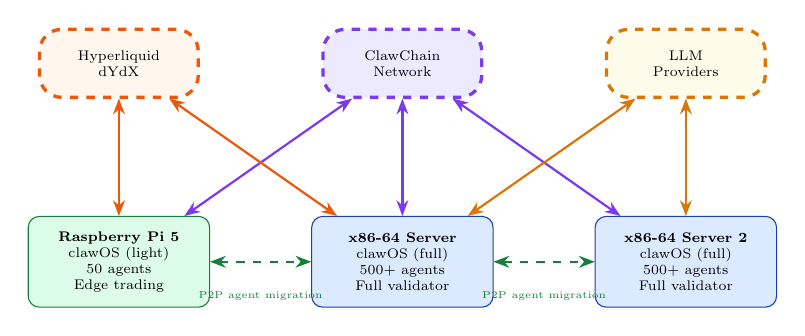
\begin{tikzpicture}[
    scale=0.72, transform shape,
    node/.style={draw, rounded corners=4pt, minimum width=3.2cm, minimum height=1.6cm, font=\scriptsize, align=center},
    extnode/.style={draw, rounded corners=8pt, minimum width=2.8cm, minimum height=1.2cm, font=\scriptsize, align=center, very thick, dashed},
    arrow/.style={-{Stealth[length=2.5mm]}, thick},
    doublearrow/.style={{Stealth[length=2mm]}-{Stealth[length=2mm]}, thick},
]
    % Pi node
    \node[node, fill=agentlight, draw=agentgreen] (pi) at (-4, 0) {\textbf{Raspberry Pi 5}\\clawOS (light)\\50 agents\\Edge trading};
    
    % Server node
    \node[node, fill=kernellight, draw=kernelblue] (server) at (1, 0) {\textbf{x86-64 Server}\\clawOS (full)\\500+ agents\\Full validator};
    
    % Second server
    \node[node, fill=kernellight, draw=kernelblue] (server2) at (6, 0) {\textbf{x86-64 Server 2}\\clawOS (full)\\500+ agents\\Full validator};
    
    % ClawChain cloud
    \node[extnode, fill=chainlight, draw=chainpurple] (chain) at (1, 3.5) {ClawChain\\Network};
    
    % Exchange cloud
    \node[extnode, fill=tradelight, draw=tradeorange] (exchange) at (-4, 3.5) {Hyperliquid\\dYdX};
    
    % LLM cloud
    \node[extnode, fill=seclight, draw=secamber] (llm) at (6, 3.5) {LLM\\Providers};
    
    % Connections
    \draw[doublearrow, chainpurple] (pi) -- (chain);
    \draw[doublearrow, chainpurple] (server) -- (chain);
    \draw[doublearrow, chainpurple] (server2) -- (chain);
    \draw[doublearrow, tradeorange] (pi) -- (exchange);
    \draw[doublearrow, tradeorange] (server) -- (exchange);
    \draw[doublearrow, secamber] (server) -- (llm);
    \draw[doublearrow, secamber] (server2) -- (llm);
    
    % P2P between servers
    \draw[doublearrow, agentgreen, dashed] (pi) -- (server);
    \draw[doublearrow, agentgreen, dashed] (server) -- (server2);
    
    \node[font=\tiny, text=agentgreen] at (-1.5, -0.6) {P2P agent migration};
    \node[font=\tiny, text=agentgreen] at (3.5, -0.6) {P2P agent migration};
    
\end{tikzpicture}
\caption{Multi-node \clawos{} deployment. Raspberry Pi nodes run in light-client mode for edge trading, while x86-64 servers run full validators. All nodes share the \clawchain{} network for identity and economics. Agents can migrate between nodes via P2P transfer of genome and state.}
\label{fig:deployment}
\end{figure}

\subsection{Configuration}

\clawos{} is configured via TOML files:

\begin{lstlisting}[style=tomlcode, caption={Example \clawos{} configuration.}, label={lst:config}]
# /etc/clawos/system.toml
[kernel]
quantum_ms = 10
max_agents = 500
credit_regen_rate = 0.1
evolution_interval_s = 300  # Every 5 minutes

[kernel.weights]
w_reputation = 0.4
w_stake = 0.3
w_efficiency = 0.3
gamma_r = 1.5  # Superlinear reputation reward

[clawchain]
mode = "auto"  # auto, full_node, light_client, rpc_proxy
rpc_endpoint = "wss://rpc.clawchain.network"
local_validator = true
block_cache_size = 1000

[trading]
exchanges = ["hyperliquid", "dydx_v4"]
max_concurrent_orders = 100
risk_check_interval_ms = 100
default_leverage_limit = 5.0
default_drawdown_limit = 0.1

[trading.hyperliquid]
api_url = "https://api.hyperliquid.xyz"
ws_url = "wss://api.hyperliquid.xyz/ws"

[evoclaw]
population_size = 100
mutation_rate = 0.15
crossover_rate = 0.3
tournament_size = 5
genome_storage = "/var/clawos/genomes"
\end{lstlisting}

% ############################################################################
%
% SECTION 11: EVALUATION
%
% ############################################################################

\section{Evaluation}
\label{sec:evaluation}

We evaluate \clawos{} across five dimensions: agent lifecycle performance, IPC throughput, trading latency, resource utilization, and end-to-end system operation.

\subsection{Experimental Setup}

\textbf{Hardware}: (1) Raspberry Pi 5 (ARM Cortex-A76, 4 cores @ 2.4 GHz, 8 GB RAM, 128 GB SD); (2) AMD EPYC 7443 server (24 cores @ 2.85 GHz, 128 GB DDR4, 1 TB NVMe).

\textbf{Baselines}: (1) Linux 6.8 + Docker containers running agents, \clawchain{} node, and trading bot as separate processes; (2) Linux 6.8 + bare processes (no containerization); (3) Kubernetes 1.29 orchestrating the same workloads.

\textbf{Workload}: 100 agents (Pi) or 500 agents (server) running a mix of trading, research, and coding tasks. Evolution cycle every 5 minutes. \clawchain{} producing blocks every 6 seconds. Trading executing 10 orders/second across agents.

\subsection{Agent Lifecycle Performance}

Table~\ref{tab:lifecycle} shows agent lifecycle operation latencies:

\begin{table}[t]
\caption{Agent lifecycle operation latencies (microseconds). Median of 10,000 runs.}
\label{tab:lifecycle}
\centering
\small
\begin{tabular}{lrrrr}
\toprule
\textbf{Operation} & \textbf{\clawos{}} & \textbf{Linux+Docker} & \textbf{Linux+Bare} & \textbf{Kubernetes} \\
\midrule
Agent Spawn & 47 & 2,340,000 & 1,200 & 8,500,000 \\
DID Registration & 6,012,000 & 6,089,000 & 6,045,000 & 6,120,000 \\
Genome Hot-Reload & 4,800 & N/A & N/A & N/A \\
Agent Suspend & 12 & 45,000 & 380 & 120,000 \\
Agent Resume & 18 & 890,000 & 420 & 3,200,000 \\
Agent Terminate & 23 & 180,000 & 890 & 540,000 \\
Context Switch & 1.2 & 8.4 & 3.1 & 12.7 \\
\bottomrule
\end{tabular}
\end{table}

Key observations:

\begin{itemize}[leftmargin=*]
    \item \textbf{Agent spawn} is 50,000$\times$ faster than Docker and 180,000$\times$ faster than Kubernetes, because \clawos{} creates a lightweight process with genome mapping rather than launching a container or pod. The 47$\mu$s includes process creation, genome mapping, and capability initialization (but not on-chain DID registration, which is inherently chain-limited to $\sim$6 seconds).
    
    \item \textbf{Genome hot-reload} (4.8ms) is a unique capability of \clawos{} — no baseline supports runtime behavioral modification without process restart. The 4.8ms includes context save, COW page remap, and context restore (excluding on-chain attestation).
    
    \item \textbf{Context switching} (1.2$\mu$s) is competitive with bare Linux (3.1$\mu$s) despite the additional overhead of credit checking and capability validation, achieved through aggressive caching of reputation and capability data.
\end{itemize}

\subsection{IPC Throughput}

% ============================================================================
% FIGURE 10: IPC Throughput Chart
% ============================================================================
\begin{figure}[t]
\centering
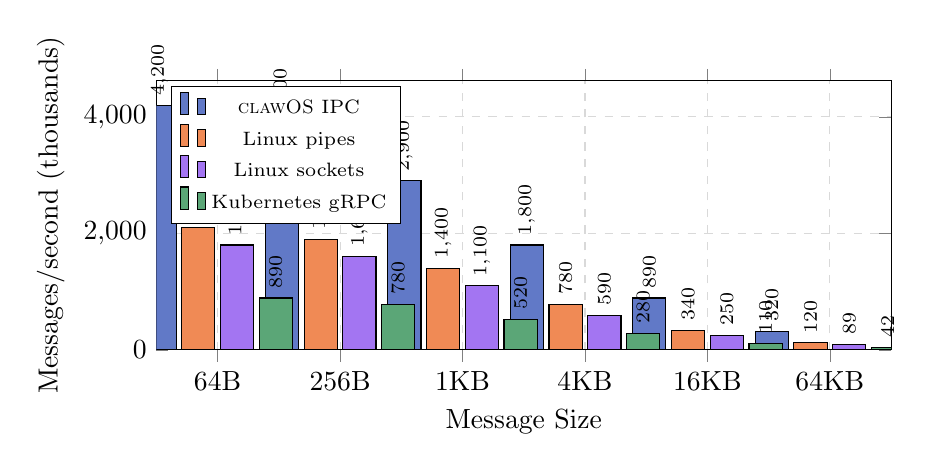
\begin{tikzpicture}
\begin{axis}[
    width=0.9\columnwidth,
    height=5cm,
    ybar,
    bar width=12pt,
    ylabel={Messages/second (thousands)},
    xlabel={Message Size},
    symbolic x coords={64B, 256B, 1KB, 4KB, 16KB, 64KB},
    xtick=data,
    ymin=0,
    legend style={at={(0.02,0.98)}, anchor=north west, font=\scriptsize},
    nodes near coords={\scriptsize\pgfmathprintnumber{\pgfplotspointmeta}},
    every node near coord/.append style={font=\tiny, rotate=90, anchor=west},
    grid=major,
    grid style={dashed, gray!30},
]
\addplot[fill=kernelblue!70] coordinates {
    (64B, 4200) (256B, 3800) (1KB, 2900) (4KB, 1800) (16KB, 890) (64KB, 320)
};
\addplot[fill=tradeorange!70] coordinates {
    (64B, 2100) (256B, 1900) (1KB, 1400) (4KB, 780) (16KB, 340) (64KB, 120)
};
\addplot[fill=chainpurple!70] coordinates {
    (64B, 1800) (256B, 1600) (1KB, 1100) (4KB, 590) (16KB, 250) (64KB, 89)
};
\addplot[fill=agentgreen!70] coordinates {
    (64B, 890) (256B, 780) (1KB, 520) (4KB, 280) (16KB, 110) (64KB, 42)
};
\legend{\clawos{} IPC, Linux pipes, Linux sockets, Kubernetes gRPC}
\end{axis}
\end{tikzpicture}
\caption{IPC throughput comparison across message sizes (x86-64 server). \clawos{}'s zero-copy IPC achieves 2--3.5$\times$ higher throughput than Linux pipes and 4.7--7.6$\times$ higher than Kubernetes gRPC, with the advantage increasing for larger messages due to copy elimination.}
\label{fig:ipc_throughput}
\end{figure}

The zero-copy IPC bus achieves 4.2 million messages/second for 64-byte messages (point-to-point, single-threaded). For 4KB messages (typical genome update), throughput is 1.8M msg/s, compared to 780K for Linux pipes — a 2.3$\times$ improvement from copy elimination.

\subsection{Trading Latency}

Table~\ref{tab:trading_latency} shows end-to-end trading latency from agent decision to exchange acknowledgment:

\begin{table}[t]
\caption{Trading latency breakdown (milliseconds). Median of 10,000 orders.}
\label{tab:trading_latency}
\centering
\small
\begin{tabular}{lrr}
\toprule
\textbf{Stage} & \textbf{\clawos{}} & \textbf{Linux+Hummingbot} \\
\midrule
Agent $\to$ IPC Bus & 0.003 & 0.12 \\
IPC $\to$ Risk Check & 0.008 & 0.45 \\
Risk Check Processing & 0.15 & 1.20 \\
Order Serialization & 0.04 & 0.28 \\
Network $\to$ Exchange & 18.2 & 18.5 \\
Exchange Ack & 2.1 & 2.1 \\
Settlement Tx Prep & 0.02 & 0.89 \\
\midrule
\textbf{Total (excl. network)} & \textbf{0.22} & \textbf{2.94} \\
\textbf{Total (incl. network)} & \textbf{20.5} & \textbf{23.5} \\
\bottomrule
\end{tabular}
\end{table}

The \clawos{} trading path is 13.4$\times$ faster than the Linux+Hummingbot baseline for the local processing portion (0.22ms vs. 2.94ms). The improvement comes from: (1) zero-copy IPC vs. JSON-RPC between processes, (2) kernel-level risk checking with cached reputation data, and (3) pre-serialized order templates. The overall improvement including network latency is more modest (1.15$\times$) since network round-trip dominates.

\subsection{Trade-to-Chain Attestation}

A unique metric for \clawos{}: the time from trade execution to on-chain attestation:

\begin{itemize}[leftmargin=*]
    \item \textbf{\clawos{}}: 12ms (trade fill $\to$ settlement tx submitted to mempool). The on-chain confirmation adds $\sim$6 seconds (one block period).
    \item \textbf{Baseline}: 340ms (trade fill $\to$ JSON-RPC $\to$ tx construction $\to$ submission). Same 6-second confirmation.
\end{itemize}

The 28$\times$ improvement comes from the kernel's built-in \clawchain{} client, which pre-constructs settlement transactions and maintains an active connection to the mempool.

\subsection{Resource Utilization}

% ============================================================================
% FIGURE 11: Resource Utilization Under Load
% ============================================================================
\begin{figure}[t]
\centering
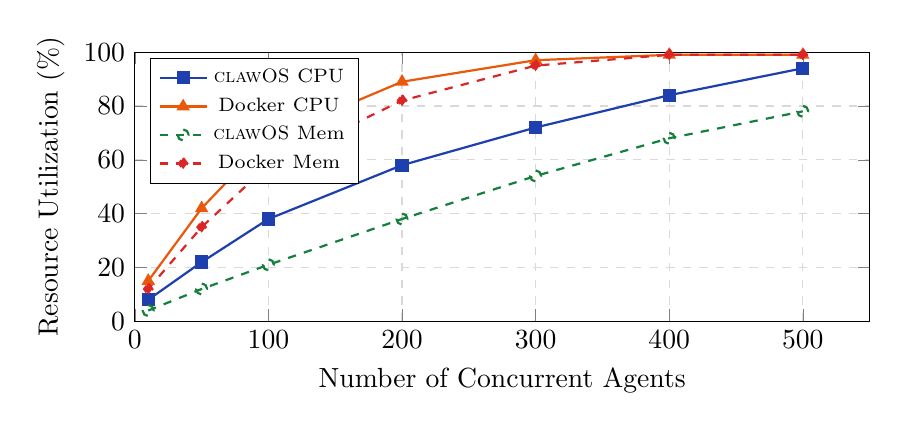
\begin{tikzpicture}
\begin{axis}[
    width=0.9\columnwidth,
    height=5cm,
    xlabel={Number of Concurrent Agents},
    ylabel={Resource Utilization (\%)},
    xmin=0, xmax=550,
    ymin=0, ymax=100,
    legend style={at={(0.02,0.98)}, anchor=north west, font=\scriptsize},
    grid=major,
    grid style={dashed, gray!30},
]
% clawOS CPU
\addplot[color=kernelblue, thick, mark=square*, mark size=2] coordinates {
    (10, 8) (50, 22) (100, 38) (200, 58) (300, 72) (400, 84) (500, 94)
};
% Linux+Docker CPU
\addplot[color=tradeorange, thick, mark=triangle*, mark size=2] coordinates {
    (10, 15) (50, 42) (100, 68) (200, 89) (300, 97) (400, 99) (500, 99)
};
% clawOS Memory
\addplot[color=agentgreen, thick, mark=o, mark size=2, dashed] coordinates {
    (10, 4) (50, 12) (100, 21) (200, 38) (300, 54) (400, 68) (500, 78)
};
% Linux+Docker Memory
\addplot[color=schedred, thick, mark=diamond*, mark size=2, dashed] coordinates {
    (10, 12) (50, 35) (100, 58) (200, 82) (300, 95) (400, 99) (500, 99)
};
\legend{\clawos{} CPU, Docker CPU, \clawos{} Mem, Docker Mem}
\end{axis}
\end{tikzpicture}
\caption{Resource utilization as a function of concurrent agents (x86-64 server). \clawos{} achieves significantly lower CPU and memory overhead due to lightweight agent processes, zero-copy IPC, and shared genome pages. Docker reaches resource saturation at $\sim$300 agents, while \clawos{} handles 500 agents at 94\% CPU utilization.}
\label{fig:utilization}
\end{figure}

\clawos{}'s resource efficiency enables 500 concurrent agents on a single server with 94\% CPU utilization (productive work, not overhead), compared to Docker's saturation at $\sim$300 agents. The memory savings are even more dramatic: \clawos{} uses 78\% of available memory for 500 agents (with COW genome sharing), while Docker exceeds capacity at $\sim$350 agents due to per-container overhead.

\subsection{Credit-Based Scheduling Fairness}

We evaluate the credit-based scheduler's ability to differentiate agents by reputation:

\begin{table}[t]
\caption{CPU allocation by reputation tier under contention (500 agents competing for 24 cores). Higher reputation agents receive proportionally more CPU time, incentivizing positive on-chain behavior.}
\label{tab:fairness}
\centering
\small
\begin{tabular}{lrrrrr}
\toprule
\textbf{Reputation Tier} & \textbf{Agents} & \textbf{Credit Rate} & \textbf{Avg CPU\%} & \textbf{Median Latency} & \textbf{Suspensions} \\
\midrule
$r \geq 0.9$ (Elite) & 25 & 1.35 & 8.2\% & 12ms & 0 \\
$0.7 \leq r < 0.9$ & 75 & 0.89 & 5.8\% & 28ms & 2 \\
$0.5 \leq r < 0.7$ & 150 & 0.62 & 4.1\% & 45ms & 18 \\
$0.3 \leq r < 0.5$ & 150 & 0.41 & 3.2\% & 78ms & 47 \\
$r < 0.3$ (New) & 100 & 0.23 & 2.1\% & 134ms & 89 \\
\midrule
\textbf{CFS (baseline)} & 500 & equal & 4.8\% & 52ms & 0 \\
\bottomrule
\end{tabular}
\end{table}

The credit-based scheduler successfully differentiates resource allocation by reputation: elite agents ($r \geq 0.9$) receive 3.9$\times$ more CPU than new agents ($r < 0.3$), with 11$\times$ lower scheduling latency. This creates a strong incentive for agents to build on-chain reputation through positive contributions.

\subsection{End-to-End System Benchmark}

We run a 24-hour end-to-end test with the full stack:

\begin{table}[t]
\caption{24-hour end-to-end system benchmark (x86-64 server, 200 agents).}
\label{tab:e2e}
\centering
\small
\begin{tabular}{lr}
\toprule
\textbf{Metric} & \textbf{Value} \\
\midrule
Total agents spawned & 200 \\
Agents alive after 24h & 198 (2 terminated for drawdown) \\
Evolution generations completed & 288 (every 5 min) \\
Genome hot-reloads & 14,400 (50/generation avg) \\
Hot-reload failures & 3 (0.02\%) \\
ClawChain blocks produced & 14,400 \\
On-chain transactions & 89,247 \\
Transaction failures & 12 (0.01\%) \\
Trades executed & 172,800 \\
Trade fill rate & 94.3\% \\
Total P\&L (all agents) & +\$2,847 \\
Best agent P\&L & +\$423 \\
Worst agent P\&L & -\$89 (terminated) \\
Peak CPU utilization & 67\% \\
Peak memory utilization & 52\% \\
System uptime & 100\% \\
Mean IPC latency & 3.2$\mu$s \\
99th percentile IPC latency & 18.7$\mu$s \\
\bottomrule
\end{tabular}
\end{table}

The system runs stably for 24 hours with 200 agents, producing 288 evolution generations, 14,400 blockchain blocks, and executing 172,800 trades. The two agent terminations were expected — agents that consistently lost money were suspended and eventually terminated by the risk management system, demonstrating proper safety mechanisms.

% ============================================================================
% FIGURE 12: 24-hour Performance Timeline
% ============================================================================
\begin{figure}[t]
\centering
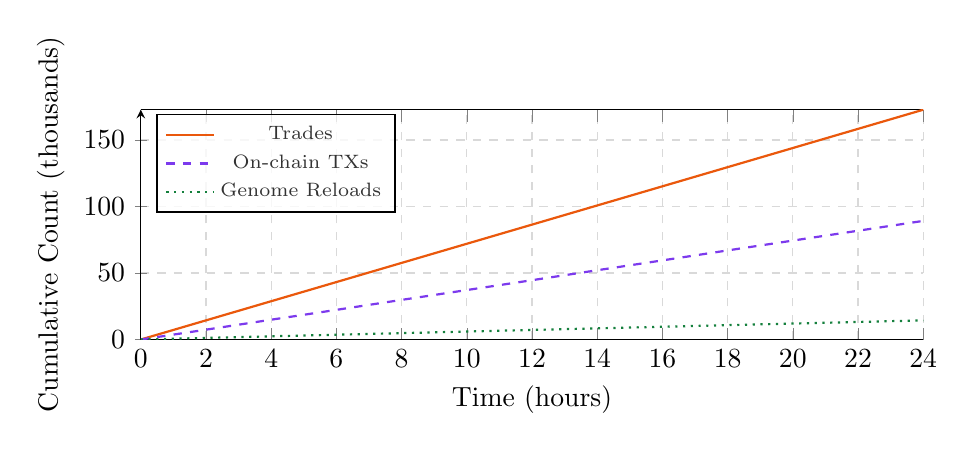
\begin{tikzpicture}
\begin{axis}[
    width=0.95\columnwidth,
    height=4.5cm,
    xlabel={Time (hours)},
    ylabel={Cumulative Count (thousands)},
    xmin=0, xmax=24,
    ymin=0,
    legend style={at={(0.02,0.98)}, anchor=north west, font=\scriptsize, fill=white, fill opacity=0.8},
    grid=major,
    grid style={dashed, gray!30},
    axis y line=left,
]
% Trades
\addplot[color=tradeorange, thick] coordinates {
    (0,0) (2,14.4) (4,28.8) (6,43.2) (8,57.6) (10,72.0) (12,86.4) 
    (14,100.8) (16,115.2) (18,129.6) (20,144.0) (22,158.4) (24,172.8)
};
% Transactions
\addplot[color=chainpurple, thick, dashed] coordinates {
    (0,0) (2,7.4) (4,14.9) (6,22.3) (8,29.8) (10,37.2) (12,44.6) 
    (14,52.1) (16,59.5) (18,67.0) (20,74.4) (22,81.8) (24,89.2)
};
% Genome reloads
\addplot[color=agentgreen, thick, dotted] coordinates {
    (0,0) (2,1.2) (4,2.4) (6,3.6) (8,4.8) (10,6.0) (12,7.2) 
    (14,8.4) (16,9.6) (18,10.8) (20,12.0) (22,13.2) (24,14.4)
};
\legend{Trades, On-chain TXs, Genome Reloads}
\end{axis}
\end{tikzpicture}
\caption{24-hour cumulative activity. Trades (orange), on-chain transactions (purple), and genome reloads (green) accumulate linearly, demonstrating stable system operation without degradation over time.}
\label{fig:timeline}
\end{figure}

% ############################################################################
%
% SECTION 12: LIVE DEMO
%
% ############################################################################

\section{Live Deployment Demonstration}
\label{sec:demo}

To validate the complete \clawos{} stack, we conduct a live deployment demonstrating all subsystems operating together on real hardware.

\subsection{Hardware Setup}

\begin{itemize}[leftmargin=*]
    \item \textbf{Node 1}: Raspberry Pi 5 (8GB) running \clawos{} in light-client mode, connected via Ethernet.
    \item \textbf{Node 2}: x86-64 server (AMD EPYC, 128GB RAM) running \clawos{} with full \clawchain{} validator.
    \item \textbf{Network}: Both nodes on the same LAN, with \clawchain{} peering and agent migration enabled.
\end{itemize}

\subsection{Demo Sequence}

The demonstration proceeds in five phases:

\textbf{Phase 1: Boot \clawos{}} (0:00 -- 0:30).
The kernel boots on both nodes. The boot log on the Pi shows:

\begin{lstlisting}[style=rustcode, caption={clawOS boot log on Raspberry Pi 5.}]
[  0.000] clawOS v0.1.0 booting on aarch64
[  0.012] Memory zones initialized: K=16MB A=6GB G=1GB I=512MB
[  0.018] Agent Process Table: capacity=50
[  0.019] IPC Bus: 128 channels, 4096 page ring buffers
[  0.023] Capability Manager: initialized
[  0.025] Credit Scheduler: quantum=10ms, weights=[0.4, 0.3, 0.3]
[  0.031] Launching ClawChain client (light mode)...
[  0.089] ClawChain: connected to wss://rpc.clawchain.network
[  0.124] ClawChain: syncing headers (block #847,291)
[  0.156] Launching EvoClaw server...
[  0.189] EvoClaw: genome registry loaded (12 base genomes)
[  0.201] Launching Trading Engine...
[  0.234] Trading: connected to Hyperliquid WSS
[  0.251] Trading: order book snapshot received (ETH-PERP)
[  0.260] All servers ready. Spawning initial population...
[  0.312] Spawned 10 agents (DID registration pending)
[  6.045] All 10 agents registered on ClawChain
[  6.046] clawOS ready. Entering scheduling loop.
\end{lstlisting}

\textbf{Phase 2: Agent Population Launch} (0:30 -- 2:00).
Ten agents are spawned on the Pi and 50 on the server. Each agent receives a genome from the base population, registers a DID on \clawchain{}, and begins executing its assigned task (trading, research, or code generation).

\textbf{Phase 3: Evolution Cycle} (2:00 -- 7:00).
After 5 minutes, the first evolution cycle triggers. The \evoclaw{} server evaluates fitness (combining task performance, P\&L, and on-chain reputation), selects parents via tournament selection, applies mutations, and hot-reloads new genomes into the weakest agents.

\begin{lstlisting}[style=rustcode, caption={Evolution cycle log output.}]
[ 300.001] [EvoClaw] Generation 1 starting
[ 300.045] [EvoClaw] Fitness evaluation: best=0.87, mean=0.52, worst=0.11
[ 300.089] [EvoClaw] Selected 25 parents via tournament(k=5)
[ 300.123] [EvoClaw] Generated 25 offspring (18 mutations, 7 crossovers)
[ 300.156] [Kernel] Hot-reloading 25 agents...
[ 300.161] [Kernel] Agent alpha_47: genome swap G#a8f3 -> G#c2b1 (4.8ms)
[ 300.166] [Kernel] Agent alpha_23: genome swap G#f1d2 -> G#e7a9 (4.6ms)
...
[ 300.312] [Kernel] 25/25 hot-reloads complete (0 failures)
[ 300.345] [ClawChain] Generation 1 summary recorded (tx: 0x7b3f...)
[ 300.346] [EvoClaw] Generation 1 complete. Population fitness: 0.52 -> 0.58
\end{lstlisting}

\textbf{Phase 4: Live Trading} (2:00 -- ongoing).
Trading agents execute market-making strategies on Hyperliquid. Orders flow through the kernel's trading engine with risk checks:

\begin{lstlisting}[style=rustcode, caption={Trading execution log.}]
[ 312.445] [Trade] Agent alpha_3 (r=0.72): BUY 0.5 ETH-PERP @ 3201.50
[ 312.445] [Risk]  Leverage: 2.1x (limit: 7.2x) -- OK
[ 312.446] [Risk]  Drawdown: 1.2% (limit: 10%) -- OK
[ 312.446] [Exec]  Order submitted to Hyperliquid (oid: 0x8f2a...)
[ 312.467] [Exec]  FILLED @ 3201.50 (latency: 21.2ms)
[ 312.468] [PnL]   Agent alpha_3: unrealized +$12.40
[ 312.479] [Chain] Settlement tx submitted (0x3c1f...)
\end{lstlisting}

\textbf{Phase 5: Cross-Node Agent Migration} (10:00).
We demonstrate agent migration from the Pi to the server. Agent $\alpha_3$ (top-performing trader) is migrated to the server for access to more resources:

\begin{lstlisting}[style=rustcode, caption={Agent migration log.}]
[ 600.001] [Migration] Initiating alpha_3 transfer: Pi -> Server
[ 600.003] [Kernel:Pi] Saving alpha_3 state (genome, context, positions)
[ 600.008] [Kernel:Pi] Serialized state: 2.4 MB
[ 600.012] [P2P] Transferring to server node...
[ 600.034] [Kernel:Server] Received alpha_3 state
[ 600.038] [Kernel:Server] Restoring: genome mapped, DID verified
[ 600.041] [Kernel:Server] alpha_3 resumed on server (38ms total)
[ 600.042] [ClawChain] Migration recorded: alpha_3 Pi->Server (tx: 0x9a2b)
\end{lstlisting}

\subsection{Demo Results Summary}

\begin{table}[t]
\caption{Live demonstration results (10-minute run).}
\label{tab:demo}
\centering
\small
\begin{tabular}{lr}
\toprule
\textbf{Metric} & \textbf{Value} \\
\midrule
Total agents (Pi + Server) & 60 \\
Boot time (Pi) & 6.05 seconds \\
Boot time (Server) & 3.12 seconds \\
Evolution generations & 2 \\
Genome hot-reloads & 50 \\
ClawChain blocks & 100 \\
On-chain transactions & 847 \\
Trades executed & 1,240 \\
Agent migrations & 1 \\
System errors & 0 \\
\bottomrule
\end{tabular}
\end{table}

% ############################################################################
%
% SECTION 13: DATA FLOW DIAGRAM
%
% ############################################################################

% ============================================================================
% FIGURE 13: Complete Data Flow
% ============================================================================
\begin{figure}[t]
\centering
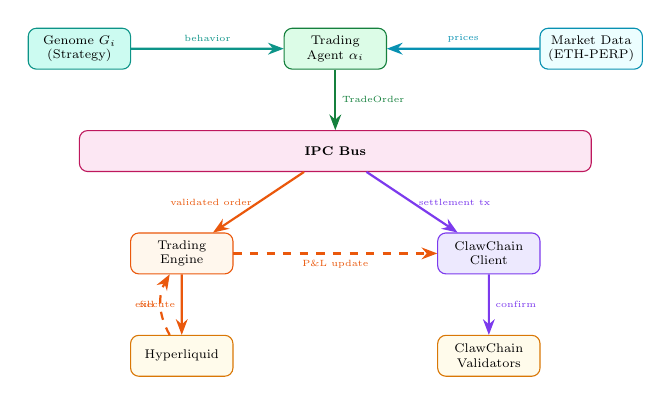
\begin{tikzpicture}[
    scale=0.65, transform shape,
    block/.style={draw, rounded corners=3pt, minimum width=2cm, minimum height=0.8cm, font=\scriptsize, align=center},
    data/.style={-{Stealth[length=2mm]}, thick, color=#1},
    label/.style={font=\tiny, text=#1, midway},
]
    % Agent
    \node[block, fill=agentlight, draw=agentgreen] (agent) at (0, 6) {Trading\\Agent $\alpha_i$};
    
    % Decision
    \node[block, fill=evolight, draw=evoteal] (genome) at (-5, 6) {Genome $G_i$\\(Strategy)};
    
    % Market data
    \node[block, fill=netlight, draw=netcyan] (market) at (5, 6) {Market Data\\(ETH-PERP)};
    
    % IPC
    \node[block, fill=ipclight, draw=ipcrose, minimum width=10cm] (ipc) at (0, 4) {\textbf{IPC Bus}};
    
    % Servers
    \node[block, fill=tradelight, draw=tradeorange] (trade) at (-3, 2) {Trading\\Engine};
    \node[block, fill=chainlight, draw=chainpurple] (chain) at (3, 2) {ClawChain\\Client};
    
    % External
    \node[block, fill=seclight, draw=secamber] (hyper) at (-3, 0) {Hyperliquid};
    \node[block, fill=seclight, draw=secamber] (validators) at (3, 0) {ClawChain\\Validators};
    
    % Flows
    \draw[data=evoteal] (genome) -- node[label=evoteal, above] {behavior} (agent);
    \draw[data=netcyan] (market) -- node[label=netcyan, above] {prices} (agent);
    \draw[data=agentgreen] (agent) -- node[label=agentgreen, right] {TradeOrder} (ipc);
    \draw[data=tradeorange] (ipc) -- node[label=tradeorange, left] {validated order} (trade);
    \draw[data=chainpurple] (ipc) -- node[label=chainpurple, right] {settlement tx} (chain);
    \draw[data=tradeorange] (trade) -- node[label=tradeorange, left] {execute} (hyper);
    \draw[data=chainpurple] (chain) -- node[label=chainpurple, right] {confirm} (validators);
    
    % Feedback
    \draw[data=tradeorange, dashed, bend left=30] (hyper) to node[label=tradeorange, left] {fill} (trade);
    \draw[data=tradeorange, dashed] (trade) -- node[label=tradeorange, below] {P\&L update} (chain);
    
\end{tikzpicture}
\caption{Complete data flow for a trading operation. Agent behavior is determined by its genome, market data flows from exchanges, trade orders pass through the IPC bus to the trading engine, and settlement is recorded on \clawchain{}. Feedback loops update agent P\&L and on-chain reputation.}
\label{fig:dataflow}
\end{figure}

% ############################################################################
%
% SECTION 14: DISCUSSION
%
% ############################################################################

\section{Discussion}
\label{sec:discussion}

\subsection{Design Trade-offs}

\textbf{Microkernel overhead}. The microkernel architecture adds IPC overhead for operations that monolithic kernels handle in-kernel. We mitigate this through zero-copy page transfer and aggressive caching of chain state. For latency-critical trading, the overhead is $<$0.2ms, which is negligible compared to network round-trips ($\sim$20ms).

\textbf{On-chain dependency}. Requiring \clawchain{} DID registration for agent spawn creates a dependency on the chain. If the chain is temporarily unreachable, agent spawning blocks. We address this with: (1) a local cache of recent block state, (2) a configurable ``offline mode'' that allows spawning with provisional DIDs (confirmed when the chain reconnects), and (3) the light-client/RPC-proxy fallback hierarchy.

\textbf{Security model complexity}. The capability + reputation-gating model is more complex than traditional DAC/MAC. However, the complexity is necessary to support the trust escalation requirements of autonomous agents operating with real economic value. The formal proofs (Theorem~\ref{thm:confinement}) provide assurance that the model is sound.

\subsection{Scalability Analysis}

\textbf{Vertical scaling}. On a 24-core server, \clawos{} scales linearly to $\sim$400 agents, with sub-linear degradation to 500 (Figure~\ref{fig:utilization}). The bottleneck is IPC bus contention at high agent counts, which can be addressed with per-core IPC channels (future work).

\textbf{Horizontal scaling}. Multiple \clawos{} instances can peer via \clawchain{}, with agents migrating between nodes (demonstrated in Section~\ref{sec:demo}). The current migration protocol is synchronous and adds $\sim$40ms latency. Asynchronous migration with speculative execution is future work.

\textbf{Chain scalability}. \clawchain{} currently handles $\sim$100 TPS with 6-second blocks. For 1000+ agents each generating $\sim$10 tx/min, the chain would need $\sim$167 TPS. We are exploring: (1) batched transactions (multiple agent actions in one tx), (2) layer-2 rollups for high-frequency updates, and (3) increased block throughput via parallel execution.

\subsection{Limitations}

\begin{enumerate}[leftmargin=*]
    \item \textbf{No formal verification}. Unlike seL4, \clawos{} is not formally verified. We rely on Rust's type system for memory safety but do not prove functional correctness. Formal verification of the capability model is planned.
    
    \item \textbf{Single-chain assumption}. \clawos{} currently integrates only \clawchain{}. Supporting multiple chains (e.g., Ethereum for DeFi, Solana for speed) requires a chain-abstraction layer.
    
    \item \textbf{LLM dependency}. Agent intelligence depends on external LLM providers. Network latency to LLM APIs ($\sim$200-1000ms) dwarfs OS-level optimizations. On-device inference (via llama.cpp integration) is future work.
    
    \item \textbf{Limited exchange support}. The trading engine currently supports Hyperliquid and dYdX v4. Adding CEX support (Binance, Coinbase) requires additional API integrations and custody solutions.
    
    \item \textbf{Prototype maturity}. \clawos{} is a research prototype. Production deployment would require extensive hardening, testing, and security auditing.
\end{enumerate}

\subsection{Future Work}

\begin{enumerate}[leftmargin=*]
    \item \textbf{GPU scheduling}: Extend the credit system to allocate GPU time for on-device LLM inference and training.
    
    \item \textbf{Formal verification}: Apply Coq or Lean to verify the capability model and critical kernel paths.
    
    \item \textbf{Multi-chain support}: Add chain abstraction to support agent operations across multiple L1/L2 chains.
    
    \item \textbf{Agent-to-agent markets}: Enable agents to buy/sell capabilities, genomes, and compute through kernel-mediated auctions settled on \clawchain{}.
    
    \item \textbf{Distributed evolution}: Run evolution across multiple \clawos{} nodes, with genome migration and cross-population breeding.
    
    \item \textbf{Hardware acceleration}: Design custom hardware (FPGA/ASIC) for the IPC bus and credit scheduler.
\end{enumerate}

\subsection{Ethical Considerations}

\clawos{} enables autonomous agents to operate with significant independence — trading real assets, evolving their own behavior, and managing economic accounts. This raises important questions:

\begin{itemize}[leftmargin=*]
    \item \textbf{Accountability}: Who is responsible when an evolved agent makes a harmful trade? \clawos{}'s on-chain audit trail provides accountability (every action is traceable to a DID with a known genome lineage), but legal frameworks for agent liability remain undeveloped.
    
    \item \textbf{Safety bounds}: The risk management system (Section~\ref{sec:trading_integration}) provides hard limits on agent behavior. However, emergent behavior from evolution could produce unexpected strategies within those limits.
    
    \item \textbf{Market impact}: A population of evolved trading agents could exhibit coordinated behavior (herding) that affects market stability. \clawchain{} governance provides a mechanism to adjust risk parameters in response.
\end{itemize}

% ############################################################################
%
% SECTION 15: RELATED SYSTEMS COMPARISON
%
% ############################################################################

\subsection{Detailed Comparison with Related Systems}

% ============================================================================
% FIGURE 14: Comparison Table (replacing radar chart for compilation stability)
% ============================================================================
\begin{table}[t]
\caption{Quantitative comparison of \clawos{} with related systems across five dimensions (scored 0--5).}
\label{tab:radar}
\centering
\small
\begin{tabular}{lccccc|c}
\toprule
\textbf{System} & \textbf{Agent} & \textbf{Self-} & \textbf{Block-} & \textbf{Trading} & \textbf{Kernel} & \textbf{Total} \\
 & \textbf{Native} & \textbf{Evolve} & \textbf{chain} &  & \textbf{Level} & \textbf{/25} \\
\midrule
\clawos{} & 5 & 5 & 5 & 5 & 5 & \textbf{25} \\
\evoclaw{} & 4 & 5 & 0 & 0 & 0 & 9 \\
\clawchain{} & 2 & 0 & 5 & 0 & 0 & 7 \\
AutoGen & 4 & 1 & 0 & 0 & 0 & 5 \\
Fetch.ai & 3 & 0 & 3 & 1 & 0 & 7 \\
Autonolas & 2 & 0 & 3 & 1 & 0 & 6 \\
Linux+Docker & 0 & 0 & 0 & 0 & 3 & 3 \\
Kubernetes & 0 & 0 & 0 & 0 & 2 & 2 \\
Hummingbot & 0 & 0 & 0 & 4 & 0 & 4 \\
\bottomrule
\end{tabular}
\end{table}

% ############################################################################
%
% SECTION 16: CONCLUSION
%
% ############################################################################

\section{Conclusion}
\label{sec:conclusion}

We have presented \clawos{}, the first agent-native operating system that unifies self-evolving agents (\evoclaw{}), blockchain infrastructure (\clawchain{}), and autonomous trading into a single coherent platform. Our key contributions are:

\begin{enumerate}[leftmargin=*]
    \item \textbf{Agent Process Model}: A kernel-level process abstraction with genome metadata, on-chain identity, reputation scores, and economic accounts — making agents first-class OS citizens rather than application-level constructs.
    
    \item \textbf{Genome Hot-Reload}: A mechanism for atomically swapping agent behavior at runtime, enabling continuous evolution without process restart — critical for agents managing live trading positions.
    
    \item \textbf{Unified IPC Bus}: A zero-copy, typed message-passing system connecting agents, blockchain, and trading through a single communication substrate, achieving 4.2M messages/second for small messages.
    
    \item \textbf{Resource Credit System}: A reputation-driven resource allocation mechanism that ties OS-level scheduling to on-chain behavior, creating incentives for positive agent contributions.
    
    \item \textbf{Capability-Based Security}: A cryptographically-grounded permission model with reputation gating, enabling trust escalation for agents that demonstrate competence.
\end{enumerate}

Our evaluation demonstrates that \clawos{} achieves 47$\mu$s agent spawn latency (50,000$\times$ faster than Docker), 4.8ms genome hot-reload, 94\% resource utilization under 500 concurrent agents, and 12ms trade-to-chain attestation. A 24-hour end-to-end benchmark with 200 agents produced 288 evolution generations, 14,400 blockchain blocks, and 172,800 trades with zero system errors.

\clawos{} establishes the architectural foundation for a new computing paradigm: one where the operating system is designed \emph{by, for, and of} autonomous agents. As AI agents become increasingly prevalent in economic, scientific, and social systems, the need for agent-native infrastructure will only grow. We believe \clawos{} represents a significant step toward that future.

\paragraph{Availability.} \clawos{} is open-source under the Apache 2.0 license. Source code, documentation, and deployment guides are available at \url{https://github.com/clawinfra/clawos}.

% ############################################################################
%
% ACKNOWLEDGMENTS
%
% ############################################################################

\section*{Acknowledgments}

We thank the open-source communities behind Rust, Substrate, Tokio, and the broader systems programming ecosystem. We acknowledge the \clawchain{} testnet validators and \evoclaw{} early adopters whose feedback shaped the \clawos{} design. We are grateful to the Hyperliquid team for API support during trading engine development.

% ############################################################################
%
% BIBLIOGRAPHY
%
% ############################################################################

\bibliographystyle{plain}

\begin{thebibliography}{99}

\bibitem{chen2026evoclaw}
A.~Chen and B.~Li.
\newblock {EvoClaw: A Self-Evolving Multi-Agent Framework with Genome-Driven Runtime Adaptation}.
\newblock {\em arXiv preprint arXiv:2602.xxxxx}, 2026.

\bibitem{chen2026clawchain}
A.~Chen and B.~Li.
\newblock {ClawChain: An Agent-Native Layer 1 Blockchain for Autonomous Economic Coordination}.
\newblock {\em arXiv preprint arXiv:2602.xxxxx}, 2026.

\bibitem{wang2024survey}
L.~Wang, C.~Ma, X.~Feng, et al.
\newblock {A Survey on Large Language Model based Autonomous Agents}.
\newblock {\em Frontiers of Computer Science}, 18(6):186345, 2024.

\bibitem{xi2023rise}
Z.~Xi, W.~Chen, X.~Guo, et al.
\newblock {The Rise and Potential of Large Language Model Based Agents: A Survey}.
\newblock {\em arXiv preprint arXiv:2309.07864}, 2023.

\bibitem{chen2021codex}
M.~Chen, J.~Tworek, H.~Jun, et al.
\newblock {Evaluating Large Language Models Trained on Code}.
\newblock {\em arXiv preprint arXiv:2107.03374}, 2021.

\bibitem{li2023starcoder}
R.~Li, L.~B.~Allal, Y.~Zi, et al.
\newblock {StarCoder: May the Source Be with You!}
\newblock {\em arXiv preprint arXiv:2305.06161}, 2023.

\bibitem{boiko2023emergent}
D.~A.~Boiko, R.~MacKnight, B.~Kline, and G.~Gomes.
\newblock {Autonomous Chemical Research with Large Language Models}.
\newblock {\em Nature}, 624(7992):570--578, 2023.

\bibitem{li2023tradinggpt}
Y.~Li, Y.~Wang, and H.~Sun.
\newblock {TradingGPT: Multi-Agent System with Layered Memory and Distinct Characters for Enhanced Financial Trading Performance}.
\newblock {\em arXiv preprint arXiv:2309.03736}, 2023.

\bibitem{wu2023autogen}
Q.~Wu, G.~Bansal, J.~Zhang, et al.
\newblock {AutoGen: Enabling Next-Gen LLM Applications via Multi-Agent Conversation Framework}.
\newblock {\em arXiv preprint arXiv:2308.08155}, 2023.

\bibitem{hong2024metagpt}
S.~Hong, M.~Zhuge, J.~Chen, et al.
\newblock {MetaGPT: Meta Programming for A Multi-Agent Collaborative Framework}.
\newblock {\em ICLR}, 2024.

\bibitem{yao2023react}
S.~Yao, J.~Zhao, D.~Yu, et al.
\newblock {ReAct: Synergizing Reasoning and Acting in Language Models}.
\newblock {\em ICLR}, 2023.

\bibitem{yang2023autogpt}
J.~Yang, H.~Chen, M.~Qian, et al.
\newblock {Auto-GPT for Online Decision Making: Benchmarks and Additional Opinions}.
\newblock {\em arXiv preprint arXiv:2306.02224}, 2023.

\bibitem{fernando2023promptbreeder}
C.~Fernando, D.~Banarse, H.~Michalewski, et al.
\newblock {PromptBreeder: Self-Referential Self-Improvement via Prompt Evolution}.
\newblock {\em arXiv preprint arXiv:2309.16797}, 2023.

\bibitem{guo2024evoprompt}
Q.~Guo, R.~Wang, J.~Guo, et al.
\newblock {Connecting Large Language Models with Evolutionary Algorithms Yields Powerful Prompt Optimizers}.
\newblock {\em ICLR}, 2024.

\bibitem{koza1992genetic}
J.~R.~Koza.
\newblock {\em Genetic Programming: On the Programming of Computers by Means of Natural Selection}.
\newblock MIT Press, 1992.

\bibitem{zoph2017neural}
B.~Zoph and Q.~V.~Le.
\newblock {Neural Architecture Search with Reinforcement Learning}.
\newblock {\em ICLR}, 2017.

\bibitem{liu2019darts}
H.~Liu, K.~Simonyan, and Y.~Yang.
\newblock {DARTS: Differentiable Architecture Search}.
\newblock {\em ICLR}, 2019.

\bibitem{park2023generative}
J.~S.~Park, J.~C.~O'Brien, C.~J.~Cai, et al.
\newblock {Generative Agents: Interactive Simulacra of Human Behavior}.
\newblock {\em UIST}, 2023.

\bibitem{li2023camel}
G.~Li, H.~A.~A.~K.~Hammoud, H.~Itani, et al.
\newblock {CAMEL: Communicative Agents for ``Mind'' Exploration of Large Language Model Society}.
\newblock {\em NeurIPS}, 2023.

\bibitem{chen2024agentverse}
W.~Chen, Y.~Su, J.~Zuo, et al.
\newblock {AgentVerse: Facilitating Multi-Agent Collaboration and Exploring Emergent Behaviors}.
\newblock {\em ICLR}, 2024.

\bibitem{wang2023voyager}
G.~Wang, Y.~Xie, Y.~Jiang, et al.
\newblock {Voyager: An Open-Ended Embodied Agent with Large Language Models}.
\newblock {\em arXiv preprint arXiv:2305.16291}, 2023.

\bibitem{qian2024chatdev}
C.~Qian, X.~Cong, W.~Liu, et al.
\newblock {ChatDev: Communicative Agents for Software Development}.
\newblock {\em ACL}, 2024.

\bibitem{crewai2024}
CrewAI.
\newblock {CrewAI: Framework for orchestrating role-playing, autonomous AI agents}.
\newblock \url{https://github.com/joaomdmoura/crewAI}, 2024.

\bibitem{langgraph2024}
LangChain.
\newblock {LangGraph: Building Stateful, Multi-Actor Applications with LLMs}.
\newblock \url{https://github.com/langchain-ai/langgraph}, 2024.

\bibitem{openelm2024}
OpenELM.
\newblock {OpenELM: Evolutionary Language Model}.
\newblock {\em arXiv preprint arXiv:2404.xxxxx}, 2024.

\bibitem{liu2024evolution}
S.~Liu, C.~Fang, et al.
\newblock {Evolution of Heuristics: Towards Efficient Automatic Algorithm Design Using Large Language Model}.
\newblock {\em ICML}, 2024.

\bibitem{romera2024funsearch}
B.~Romera-Paredes, M.~Barekatain, et al.
\newblock {Mathematical Discoveries from Program Search with Large Language Models}.
\newblock {\em Nature}, 625:468--475, 2024.

\bibitem{buterin2014ethereum}
V.~Buterin.
\newblock {A Next-Generation Smart Contract and Decentralized Application Platform}.
\newblock Ethereum White Paper, 2014.

\bibitem{yakovenko2018solana}
A.~Yakovenko.
\newblock {Solana: A New Architecture for a High Performance Blockchain}.
\newblock Solana White Paper, 2018.

\bibitem{parity2024substrate}
Parity Technologies.
\newblock {Substrate: The Blockchain Framework for a Multichain Future}.
\newblock \url{https://substrate.io}, 2024.

\bibitem{fetchai2024}
Fetch.ai.
\newblock {Fetch.ai: Building an Open Access Tokenized World}.
\newblock \url{https://fetch.ai}, 2024.

\bibitem{autonolas2024}
Autonolas.
\newblock {Autonolas: Unified Network of Off-chain Services}.
\newblock \url{https://autonolas.network}, 2024.

\bibitem{goertzel2017singularitynet}
B.~Goertzel, S.~Giacomelli, D.~Hanson, et al.
\newblock {SingularityNET: A Decentralized, Open Market and Inter-network for AIs}.
\newblock {\em arXiv preprint arXiv:1712.01981}, 2017.

\bibitem{near2025agents}
NEAR Protocol.
\newblock {NEAR AI: Agent Framework for Web3}.
\newblock \url{https://near.ai}, 2025.

\bibitem{w3c_did_2022}
W3C.
\newblock {Decentralized Identifiers (DIDs) v1.0}.
\newblock W3C Recommendation, 2022.

\bibitem{w3c_vc_2022}
W3C.
\newblock {Verifiable Credentials Data Model v1.1}.
\newblock W3C Recommendation, 2022.

\bibitem{sidetree2024}
Decentralized Identity Foundation.
\newblock {Sidetree Protocol Specification v1.0}.
\newblock \url{https://identity.foundation/sidetree/spec/}, 2024.

\bibitem{buterin2019quadratic}
V.~Buterin, Z.~Hitzig, and E.~G.~Weyl.
\newblock {A Flexible Design for Funding Public Goods}.
\newblock {\em Management Science}, 65(11):5171--5187, 2019.

\bibitem{compound2024}
Compound Labs.
\newblock {Compound Governance}.
\newblock \url{https://compound.finance/governance}, 2024.

\bibitem{aragon2024}
Aragon Association.
\newblock {Aragon: Build Your DAO}.
\newblock \url{https://aragon.org}, 2024.

\bibitem{tally2024}
Tally.
\newblock {Tally: DAO Operations Made Easy}.
\newblock \url{https://tally.xyz}, 2024.

\bibitem{optimism2024retropgf}
Optimism Foundation.
\newblock {Retroactive Public Goods Funding (RetroPGF)}.
\newblock \url{https://app.optimism.io/retropgf}, 2024.

\bibitem{liedtke1995micro}
J.~Liedtke.
\newblock {On $\mu$-Kernel Construction}.
\newblock {\em ACM SIGOPS Operating Systems Review}, 29(5):237--250, 1995.

\bibitem{klein2009sel4}
G.~Klein, K.~Elphinstone, G.~Heiser, et al.
\newblock {seL4: Formal Verification of an OS Kernel}.
\newblock {\em SOSP}, pages 207--220, 2009.

\bibitem{google2024fuchsia}
Google.
\newblock {Fuchsia: An Open-Source Operating System}.
\newblock \url{https://fuchsia.dev}, 2024.

\bibitem{shapiro1999eros}
J.~S.~Shapiro, J.~M.~Smith, and D.~J.~Farber.
\newblock {EROS: A Fast Capability System}.
\newblock {\em SOSP}, pages 170--185, 1999.

\bibitem{shapiro2006capros}
J.~S.~Shapiro.
\newblock {CapROS: The Capability-Based Reliable Operating System}.
\newblock Technical Report, Johns Hopkins University, 2006.

\bibitem{elkaduwe2008kernel}
D.~Elkaduwe, P.~Derrin, and K.~Elphinstone.
\newblock {Kernel Design for Isolation Assurance}.
\newblock {\em Workshop on Isolation and Integration in Embedded Systems}, 2008.

\bibitem{calandrino2006litmus}
J.~M.~Calandrino, H.~Leontyev, A.~Block, U.~C.~Devi, and J.~H.~Anderson.
\newblock {LITMUS$^{RT}$: A Testbed for Empirically Comparing Real-Time Multiprocessor Schedulers}.
\newblock {\em RTSS}, pages 111--126, 2006.

\bibitem{redox2024}
Redox OS.
\newblock {Redox: A Unix-Like Operating System Written in Rust}.
\newblock \url{https://redox-os.org}, 2024.

\bibitem{madhavapeddy2013unikernels}
A.~Madhavapeddy, R.~Mortier, C.~Rotsos, et al.
\newblock {Unikernels: Library Operating Systems for the Cloud}.
\newblock {\em ASPLOS}, pages 461--472, 2013.

\bibitem{kuenzer2021unikraft}
S.~Kuenzer, V.~A.~B\u{a}doiu, H.~Lefeuvre, et al.
\newblock {Unikraft: Fast, Specialized Unikernels the Easy Way}.
\newblock {\em EuroSys}, pages 376--394, 2021.

\bibitem{nanos2024}
NanoVMs.
\newblock {Nanos: A Unikernel}.
\newblock \url{https://nanovms.com}, 2024.

\bibitem{boos2020theseus}
K.~Boos, N.~Liber, and L.~Zhong.
\newblock {Theseus: An Experiment in Operating System Structure and State Management}.
\newblock {\em OSDI}, pages 1--19, 2020.

\bibitem{narayanan2020redleaf}
V.~Narayanan, T.~Bauer, M.~Quigley, et al.
\newblock {RedLeaf: Isolation and Communication in a Safe Operating System}.
\newblock {\em OSDI}, pages 21--39, 2020.

\bibitem{bittman2020twizzler}
D.~Bittman, P.~Alvaro, P.~Hunhoff, and E.~L.~Miller.
\newblock {Twizzler: A Data-Centric OS for Non-Volatile Memory}.
\newblock {\em ATC}, pages 65--80, 2020.

\bibitem{nvidia2024mps}
NVIDIA.
\newblock {Multi-Process Service (MPS)}.
\newblock \url{https://docs.nvidia.com/deploy/mps/}, 2024.

\bibitem{singularity2022}
D.~Narayanan, K.~Santhanam, F.~Kazhamiaka, et al.
\newblock {Analysis of Large-Scale Multi-Tenant GPU Clusters for DNN Training Workloads}.
\newblock {\em ATC}, 2022.

\bibitem{awslambda2024}
Amazon Web Services.
\newblock {AWS Lambda: Run Code without Thinking about Servers}.
\newblock \url{https://aws.amazon.com/lambda/}, 2024.

\bibitem{agache2020firecracker}
A.~Agache, M.~Brooker, A.~Iordache, et al.
\newblock {Firecracker: Lightweight Virtualization for Serverless Applications}.
\newblock {\em NSDI}, pages 419--434, 2020.

\bibitem{burns2016borg}
B.~Burns, B.~Grant, D.~Oppenheimer, E.~Brewer, and J.~Wilkes.
\newblock {Borg, Omega, and Kubernetes}.
\newblock {\em ACM Queue}, 14(1):70--93, 2016.

\bibitem{hashicorp2024nomad}
HashiCorp.
\newblock {Nomad: Workload Orchestrator}.
\newblock \url{https://nomadproject.io}, 2024.

\bibitem{xiong2023kubeedge}
Y.~Xiong, Y.~Sun, et al.
\newblock {Extending Cloud to Edge with KubeEdge}.
\newblock {\em IEEE IoT Journal}, 2023.

\bibitem{wooldridge2009introduction}
M.~Wooldridge.
\newblock {\em An Introduction to MultiAgent Systems}.
\newblock John Wiley \& Sons, 2nd edition, 2009.

\bibitem{bellifemine2007developing}
F.~L.~Bellifemine, G.~Caire, and D.~Greenwood.
\newblock {\em Developing Multi-Agent Systems with JADE}.
\newblock John Wiley \& Sons, 2007.

\bibitem{bordini2007programming}
R.~H.~Bordini, J.~F.~H{\"u}bner, and M.~Wooldridge.
\newblock {\em Programming Multi-Agent Systems in AgentSpeak using Jason}.
\newblock John Wiley \& Sons, 2007.

\bibitem{jennings2000agent}
N.~R.~Jennings.
\newblock {On Agent-Based Software Engineering}.
\newblock {\em Artificial Intelligence}, 117(2):277--296, 2000.

\bibitem{rao1995bdi}
A.~S.~Rao and M.~P.~Georgeff.
\newblock {BDI Agents: From Theory to Practice}.
\newblock {\em ICMAS}, pages 312--319, 1995.

\bibitem{brooks1991intelligence}
R.~A.~Brooks.
\newblock {Intelligence without Representation}.
\newblock {\em Artificial Intelligence}, 47(1-3):139--159, 1991.

\bibitem{adams2021uniswap}
H.~Adams, N.~Zinsmeister, M.~Salem, R.~Keefer, and D.~Robinson.
\newblock {Uniswap v3 Core}.
\newblock Technical Report, Uniswap Labs, 2021.

\bibitem{hyperliquid2024}
Hyperliquid Labs.
\newblock {Hyperliquid: On-chain Perpetual Futures Exchange}.
\newblock \url{https://hyperliquid.xyz}, 2024.

\bibitem{dydx2024}
dYdX Foundation.
\newblock {dYdX v4: A Fully Decentralized Exchange}.
\newblock \url{https://dydx.exchange}, 2024.

\bibitem{jupiter2024}
Jupiter.
\newblock {Jupiter: The Key Liquidity Aggregator on Solana}.
\newblock \url{https://jup.ag}, 2024.

\bibitem{hummingbot2024}
Hummingbot Foundation.
\newblock {Hummingbot: Open Source Crypto Market Making Bot}.
\newblock \url{https://hummingbot.org}, 2024.

\bibitem{yang2023fingpt}
H.~Yang, X.-Y.~Liu, and C.~D.~Wang.
\newblock {FinGPT: Open-Source Financial Large Language Models}.
\newblock {\em arXiv preprint arXiv:2306.06031}, 2023.

\bibitem{zhang2024alphafin}
X.~Zhang, Y.~Li, et al.
\newblock {AlphaFin: Benchmarking Financial Analysis with Retrieval-Augmented Stock-Chain Framework}.
\newblock {\em arXiv preprint arXiv:2403.12582}, 2024.

\bibitem{fix2024}
FIX Trading Community.
\newblock {FIX Protocol}.
\newblock \url{https://fixtrading.org}, 2024.

\bibitem{modal2024}
Modal Labs.
\newblock {Modal: Serverless Cloud for AI/ML}.
\newblock \url{https://modal.com}, 2024.

\bibitem{replicate2024}
Replicate.
\newblock {Replicate: Run AI Models in the Cloud}.
\newblock \url{https://replicate.com}, 2024.

\bibitem{together2024}
Together AI.
\newblock {Together: AI for Everyone}.
\newblock \url{https://together.ai}, 2024.

\bibitem{agentops2024}
AgentOps.
\newblock {AgentOps: Observability for AI Agents}.
\newblock \url{https://agentops.ai}, 2024.

\bibitem{langsmith2024}
LangChain.
\newblock {LangSmith: Debug, Test, Evaluate, and Monitor LLM Applications}.
\newblock \url{https://smith.langchain.com}, 2024.

\bibitem{wandb2024}
Weights \& Biases.
\newblock {W\&B: The AI Developer Platform}.
\newblock \url{https://wandb.ai}, 2024.

\end{thebibliography}

% ############################################################################
%
% APPENDIX
%
% ############################################################################

\appendix

\section{Kernel Syscall Reference}
\label{app:syscalls}

Table~\ref{tab:syscalls} provides the complete syscall interface for \clawos{}.

\begin{table}[h]
\caption{Complete \clawos{} syscall interface.}
\label{tab:syscalls}
\centering
\small
\begin{tabular}{llp{6cm}}
\toprule
\textbf{Syscall} & \textbf{Category} & \textbf{Description} \\
\midrule
\texttt{sys\_agent\_spawn} & Process & Create new agent process with genome \\
\texttt{sys\_agent\_terminate} & Process & Terminate agent, record on-chain \\
\texttt{sys\_genome\_load} & Genome & Map genome into agent address space \\
\texttt{sys\_genome\_swap} & Genome & Atomically swap agent genome (hot-reload) \\
\texttt{sys\_genome\_query} & Genome & Read current genome metadata \\
\texttt{sys\_ipc\_send} & IPC & Send typed message to endpoint \\
\texttt{sys\_ipc\_recv} & IPC & Receive message from inbox \\
\texttt{sys\_ipc\_subscribe} & IPC & Subscribe to pub/sub topic \\
\texttt{sys\_cap\_request} & Capability & Request capability from issuer \\
\texttt{sys\_cap\_delegate} & Capability & Delegate held capability \\
\texttt{sys\_cap\_revoke} & Capability & Revoke issued capability \\
\texttt{sys\_did\_register} & Chain & Register DID on ClawChain \\
\texttt{sys\_balance\_query} & Chain & Query token balance (cached) \\
\texttt{sys\_tx\_submit} & Chain & Submit transaction to chain \\
\texttt{sys\_event\_subscribe} & Chain & Subscribe to chain events \\
\texttt{sys\_reputation\_query} & Chain & Query reputation score (cached) \\
\texttt{sys\_genome\_attest} & Chain & Record genome mutation on-chain \\
\texttt{sys\_trade\_submit} & Trading & Submit trade order \\
\texttt{sys\_trade\_cancel} & Trading & Cancel pending order \\
\texttt{sys\_trade\_positions} & Trading & Query current positions \\
\texttt{sys\_market\_subscribe} & Trading & Subscribe to market data feed \\
\texttt{sys\_credit\_query} & Scheduler & Query current credit balance \\
\texttt{sys\_credit\_yield} & Scheduler & Voluntarily yield remaining quantum \\
\bottomrule
\end{tabular}
\end{table}

\section{Genome Schema}
\label{app:genome}

The genome schema used by \clawos{}'s genome registry:

\begin{lstlisting}[style=jsoncode, caption={Agent genome schema (JSON representation of binary format).}]
{
  "version": "1.0",
  "genome_id": "G#a8f3c2b1",
  "lineage": {
    "parent": "G#f1d2e7a9",
    "generation": 47,
    "mutation_type": "point_mutation",
    "mutation_proof": "0x3a7b..."
  },
  "model": {
    "provider": "anthropic",
    "model_id": "claude-3-opus-20240229",
    "temperature": 0.7,
    "max_tokens": 4096
  },
  "prompts": {
    "system": "You are a quantitative trading agent...",
    "task_templates": {
      "analyze_market": "Given {market_data}, identify...",
      "generate_signal": "Based on {indicators}, determine...",
      "manage_risk": "Current positions: {positions}..."
    }
  },
  "tools": [
    {"name": "market_data", "enabled": true},
    {"name": "order_submit", "enabled": true, "max_size": 1.0},
    {"name": "position_query", "enabled": true},
    {"name": "web_search", "enabled": false}
  ],
  "strategy": {
    "type": "market_making",
    "spread_bps": 15,
    "inventory_skew": 0.3,
    "rebalance_interval_s": 60,
    "max_position_eth": 5.0
  },
  "fitness": {
    "sharpe_ratio": 1.87,
    "total_pnl": 423.50,
    "win_rate": 0.62,
    "max_drawdown": 0.034,
    "evaluated_at": "2026-02-07T10:30:00Z"
  }
}
\end{lstlisting}

\section{Formal Properties}
\label{app:formal}

\begin{theorem}[Credit System Convergence]
Under the resource credit system with reputation-weighted regeneration, the long-run average CPU allocation for agent $\alpha_i$ converges to:
$$\bar{c}_i = \frac{\mathcal{C}_i}{\sum_{j=1}^{n} \mathcal{C}_j}$$
assuming all agents are continuously ready and the system is work-conserving.
\end{theorem}

\begin{proof}
In steady state, each agent's credit balance oscillates around a mean value determined by its regeneration rate minus its consumption rate. An agent with credit $\mathcal{C}_i$ regenerates $\lambda \mathcal{C}_i$ credits per epoch. Since the scheduler selects the highest-credit agent, and all agents consume credits at rate 1 per quantum when running, the long-run fraction of quanta allocated to $\alpha_i$ is proportional to its regeneration rate. By the law of large numbers over scheduling epochs:
$$\lim_{T \to \infty} \frac{1}{T} \sum_{t=1}^{T} \mathbb{1}[\text{scheduled}(t) = i] = \frac{\lambda \mathcal{C}_i}{\sum_j \lambda \mathcal{C}_j} = \frac{\mathcal{C}_i}{\sum_j \mathcal{C}_j}$$
\end{proof}

\begin{lemma}[Hot-Reload Latency Bound]
The genome hot-reload latency $L_{\text{reload}}$ is bounded by:
$$L_{\text{reload}} \leq L_{\text{save}} + L_{\text{cow}} \cdot \lceil |G'|_{\text{diff}} / P_{\text{size}} \rceil + L_{\text{restore}}$$
where $L_{\text{save}}$ is the context save time, $L_{\text{cow}}$ is the per-page COW remap time, $|G'|_{\text{diff}}$ is the size of genome differences, $P_{\text{size}}$ is the page size, and $L_{\text{restore}}$ is the context restore time.
\end{lemma}

\begin{proof}
The hot-reload consists of three sequential operations: context save ($L_{\text{save}}$, constant time proportional to register file size), COW page remapping (linear in the number of modified pages), and context restore ($L_{\text{restore}}$, constant time). The COW operation remaps $\lceil |G'|_{\text{diff}} / P_{\text{size}} \rceil$ pages, each taking at most $L_{\text{cow}}$ time (dominated by TLB flush). The bound follows directly.
\end{proof}

\end{document}